% ============================================================================
% Functional Trust Regions (FTR): A Lagrangian Framework for
% Stability-Constrained Continual Learning
% ----------------------------------------------------------------------------
% v2 working draft. Baseline reconstructed from the compiled Research Square
% v1 preprint (DOI 10.21203/rs.3.rs-9205833/v1, posted 2026-03-25); no .tex
% source for v1 existed in the repository, only the compiled PDF, so this
% file starts as a faithful transcription and is edited in place from here.
% ============================================================================
\documentclass[11pt]{article}
\usepackage[margin=1in]{geometry}
\usepackage{cmap}
\usepackage[utf8]{inputenc}
\usepackage[T1]{fontenc}
\usepackage{amsmath,amssymb,amsfonts,amsthm}
\usepackage{graphicx}
\usepackage{booktabs}
\usepackage{multirow}
\usepackage{algorithm}
\usepackage{algorithmic}
\usepackage{hyperref}
\usepackage{xcolor}
\usepackage{natbib}
\usepackage{caption}

\newtheorem{theorem}{Theorem}
\newtheorem{proposition}{Proposition}
\newtheorem{definition}{Definition}
\newtheorem{corollary}{Corollary}

\newcommand{\R}{\mathbb{R}}
\newcommand{\E}{\mathbb{E}}
\newcommand{\eps}{\varepsilon}
\newcommand{\epsstar}{\eps^{*}}
\newcommand{\DKL}{D_{\mathrm{KL}}}

% TODO markers for content pending campaign results -- search for "TODODATA"
\newcommand{\TODODATA}[1]{\textcolor{red}{[TODODATA: #1]}}

\title{Functional Trust Regions (FTR): A Lagrangian Framework for\\
Stability-Constrained Continual Learning}
\author{
Kavya Bhand\textsuperscript{1} \quad Aadi Joshi\textsuperscript{1} \quad Vijay Rathod\textsuperscript{2} \\[4pt]
\small \textsuperscript{1}Department of Computer Engineering, Vishwakarma Institute of Technology \\
\small Pune 411037, India \\[2pt]
\small \textsuperscript{2}Department of Computer Science and Engineering (AI \& ML) \\
\small Vishwakarma Institute of Technology, Pune 411037, India \\[4pt]
\small \texttt{\{kavya.bhand0806,toaadijoshi\}@gmail.com}, \texttt{vijay.rathod@vit.edu}
}
\date{}

\makeatletter
\def\@maketitle{%
  \newpage
  \null
  \vskip 0.3em%
  \begin{center}%
  \let \footnote \thanks
    {\LARGE \@title \par}%
    \vskip 1.5em%
    {\large
      \lineskip .5em%
      \begin{tabular}[t]{c}%
        \@author
      \end{tabular}\par}%
    \vskip 1em%
    {\large \@date}%
  \end{center}%
  \par
  \vskip 1em}
\makeatother

\begin{document}
\maketitle
\let\svthefootnote\thefootnote
\let\thefootnote\relax\footnotetext{Preprint. Under review.}
\let\thefootnote\svthefootnote

\begin{abstract}
A prior study of Functional Trust Regions (FTR), a method that enforces
explicit KL-divergence constraints on functional drift during sequential
task learning, reported that the critical stability budget $\epsstar$ at
which forgetting turns catastrophic is constant across eight architectures,
concluding it reflects task structure rather than model geometry. This
account is incomplete: because the dual-ascent optimizer resets its Lagrange
multiplier at every task boundary, $\epsstar$ is mechanically co-determined
by the optimizer's own hyperparameters, not only by task or architecture.
Holding architecture and task fixed, the dual learning rate, the initial
multiplier, and the steps-per-task budget each move $\epsstar$ by more than
an order of magnitude; across six single-factor perturbations, $\epsstar$
spans roughly $1$ to $90$ on the \emph{same} model and task, a $93\times$
range that exceeds the $2.6\times$ range $\epsstar$ itself spans across
30 architectures with the schedule held fixed. This
three-dimensional sensitivity is not irreducible: it collapses
substantially onto a single ratio, $S=\lambda_{\mathrm{init}}/(\eta_\lambda N)$.
Holding $S$ fixed while independently varying its three components by up
to $5\times$ keeps $\epsstar$ within a factor of $2$--$3$, whereas changing
$S$ itself by the same factor collapses $\epsstar$ by $4$--$11\times$,
turning an intractable three-hyperparameter sensitivity into a single
number a practitioner can report and match. Holding the schedule fixed and
expanding the architecture zoo to 30 models across five representational
families (CNN, ResNet, MLP, Vision Transformer, MLP-Mixer), a hierarchical
partial-pooling model, replacing the original F-test whose own code and
reported degrees of freedom disagreed, initially estimates real,
non-negligible between-architecture structure. Applying this paper's own
diagnostic standard to its own zoo design, however, this research traces
most of that structure to two further, independently-diagnosed
data-quality issues: a
self-inflicted instance of the same schedule confound affecting four
architectures, and a curve-fitting artifact affecting two more. Correcting
both cuts the model's between-architecture variance by more than half
(from $\tau=2.13$ to $1.03$) and gives a corrected population-level
crossover of $\epsstar=11.07\pm0.25$. At this larger, adequately powered
sample, the four purely curvature-based statistics this work tests (Hessian trace,
Fisher trace, spectral norm, gradient norm) remain uncorrelated with
$\epsstar$, confirming the original curvature-irrelevance claim on grounds
its own underpowered $n=8$ test could not support, though model size shows
a small trend worth further testing. Cross-method comparison on a matched
architecture subset shows LwF exhibits the same qualitative universal
crossover while EWC and SI show none, and further robustness checks (KL
direction, task ordering, class-incremental evaluation, task granularity)
both support and further qualify the picture. A pretrained ViT-B/16 with a
LoRA adapter on Split CIFAR-100, a setting closer to how continual
learning is actually practiced, shows FTR's seed-to-seed forgetting
variance an order of magnitude tighter than the next best method, with
mean forgetting and accuracy also, by a smaller margin, the best of the
four. Together, these
results invert the original study's practical guidance: architecture-specific
tuning of the stability budget is largely unnecessary, but the dual-ascent
schedule that enforces it is not a free implementation detail, and
checking sensitivity to it, ideally by reporting $S$, belongs in the
standard protocol for Lagrangian-constrained continual learning.
\end{abstract}

\section{Introduction}
\label{sec:intro}

The fundamental challenge of continual learning is to enable neural networks
to acquire new knowledge from sequential tasks without catastrophic
interference with previously learned information \citep{mccloskey1989catastrophic,robins1995catastrophic}.
The stability-plasticity dilemma has motivated numerous approaches, including
parameter-space regularization methods such as Elastic Weight Consolidation
(EWC) \citep{kirkpatrick2017overcoming} and Synaptic Intelligence (SI)
\citep{zenke2017continual}, output-space distillation approaches like
Learning without Forgetting (LwF) \citep{li2017learning}, and memory-based
methods including experience replay \citep{lopezpaz2017gradient} and
generative replay \citep{shin2017continual}.

A central practical challenge across all these methodological families is
setting the magnitude of the stability constraint, typically represented as a
scalar hyperparameter controlling the aggressiveness of stability protection.
For EWC, practitioners must specify the Fisher coefficient. For LwF, the
distillation weight must be tuned. For replay methods, the buffer size
requires selection. Existing work suggests that these hyperparameters should
be architecture-dependent, as loss-landscape curvature varies substantially
across models of different depths, widths, and normalization strategies
\citep{keskar2016large,ghorbani2019investigation,li2018visualizing}.

This assumption is motivated by decades of work connecting loss-landscape
geometry to optimization difficulty, generalization, and robustness
\citep{novak2018sensitivity,li2018visualizing,keskar2016large}. The intuition
is compelling: models with sharper minima (higher Hessian curvature or Fisher
information) should require stronger stability pressure to prevent
catastrophic forgetting because small parameter perturbations produce large
functional changes. Conversely, models with flatter minima should tolerate
larger updates.

This research asks whether this curvature-dependent
hypothesis holds when stability is enforced as a hard constraint in function
space via KL divergence, rather than as a soft penalty in parameter space.
The constraint $\DKL(f_\theta \| f_{\mathrm{old}}) \le \eps$ directly limits
functional drift in output probability distributions, raising the question:
does the critical stability budget $\epsstar$ depend on model architecture and
loss-landscape geometry, or does it emerge as an invariant of the task
structure alone? This work additionally asks a question the constrained-continual-learning
literature has not, to this work's knowledge, posed: \emph{is $\epsstar$ in fact
determined chiefly by the constrained optimizer's own dual-ascent schedule
rather than by the model or the task at all?} Section~\ref{sec:diagnostic}
answers this second question first, because the answer determines how the
rest of the paper's architecture-independence result should be read: not as
a hyperparameter-free constant, but as a value conditional on the schedule,
whose \emph{architecture}-independence (holding that schedule fixed) is
nonetheless real and is the paper's remaining claim.

Contrary to the reading that stability
crossovers reflect task or architecture geometry alone, this research finds that the
dual-ascent optimizer's own schedule dominates: holding architecture and
task fixed, a five-fold change in the dual learning rate $\eta_\lambda$, the
initial multiplier $\lambda_{\mathrm{init}}$, or the per-task step budget
each moves $\epsstar$ by more than an order of magnitude
(Section~\ref{sec:diagnostic}), more than the $2.6\times$ range $\epsstar$
itself spans across 30 architectures with the
schedule held fixed, and more than any single robustness axis this work
tests afterward (KL direction, task ordering, class-incremental vs.\
task-incremental protocol). This three-dimensional schedule sensitivity is
not irreducible, however: Section~\ref{sec:sinvariance} shows it collapses
substantially onto a single ratio, $S=\lambda_{\mathrm{init}}/(\eta_\lambda N)$,
holding which fixed keeps $\epsstar$ within a factor of $2$--$3$ across
architectures and schedule routes, versus the order-of-magnitude range any
of its three components produces alone. Holding the schedule fixed,
$\epsstar$ remains architecture-independent in the sense that matters
operationally: no per-architecture retuning is needed, across an expanded,
30-model, five-family zoo, though a hierarchical model shows genuine (if
modest) between-architecture structure that a single reported constant
obscures (Section~\ref{sec:universality}); notably, applying this paper's
own optimizer-schedule diagnostic to its own zoo design caught a second,
self-inflicted instance of the same confound inflating that apparent
structure (Section~\ref{sec:selfconfound}).

This work makes the following contributions:
\begin{enumerate}
    \item This research identifies and directly tests a confound in Lagrangian-dual
    constrained continual learning that no prior work on
    this optimization paradigm is known to have isolated: because the dual variable is
    reset at every task boundary, the apparent stability threshold of a
    KL-constrained method is jointly determined by the optimizer's own
    schedule and by task/architecture geometry, and the schedule's effect
    can dominate (Section~\ref{sec:diagnostic}).
    \item Holding the schedule fixed, this work expands the architecture zoo from 8
    to 30 models across five representational families (CNN, ResNet, plain
    MLP, ViT, MLP-Mixer) and shows, via a hierarchical partial-pooling model,
    that $\epsstar$ is not a single universal constant as v1 claimed but has
    real, if modest, between-architecture structure; curvature-based metrics
    still fail to predict it, now with adequate statistical power to support
    that conclusion (Section~\ref{sec:universality}). This research further shows that
    part of the apparent family-level structure initially observed was
    itself a second, self-inflicted instance of the schedule confound in
    this paper's own zoo design, caught and corrected by applying its own
    diagnostic standard (Section~\ref{sec:selfconfound}), and that LwF's own
    universal crossover replicates, while EWC and SI show no reliable
    crossover at all, on this same expanded, matched architecture subset
    (Section~\ref{sec:crossmethod}). Task ordering (Section~\ref{sec:taskstructure})
    and the class-incremental protocol (Section~\ref{sec:classincremental})
    are both real, non-schedule sources of variation in $\epsstar$ that v1's
    single fixed ordering and task-incremental-only design could not surface.
    \item This research corrects a methodological error in the original F-test for
    constancy (its code computed $p$ using $df_2=1000$ while the manuscript
    reported $df=(7,7)$) with a hierarchical partial-pooling model, and shows
    the original curvature-correlation result was underpowered rather than
    confirmatory of the null (Section~\ref{sec:universality}).
    \item This work identifies and tests the specific ratio,
    $S=\lambda_{\mathrm{init}}/(\eta_\lambda N)$, that governs the
    schedule's effect on $\epsstar$, and shows that holding it fixed while
    independently varying its three components by up to $5\times$ keeps
    $\epsstar$ within a factor of $2$--$3$ across five architectures
    spanning four representational families, converting an otherwise intractable three-hyperparameter
    sensitivity into a single reportable quantity
    (Section~\ref{sec:sinvariance}).
\end{enumerate}

\section{Related Work}
\label{sec:related}

\subsection{Continual Learning Regularization}
Elastic Weight Consolidation (EWC) \citep{kirkpatrick2017overcoming} imposes
penalties on parameter changes weighted by the diagonal Fisher information
matrix, treating each parameter's importance as proportional to its
curvature contribution and protecting the parameters most responsible for
prior-task performance while leaving the rest free to adapt. It is the
most widely adopted parameter-space regularizer and the natural EWC
baseline used throughout Section~\ref{sec:crossmethod}.

Synaptic Intelligence (SI) \citep{zenke2017continual} replaces EWC's
end-of-task Fisher estimate with an online importance signal, accumulating
a path integral of each parameter's contribution to the loss reduction
along the entire training trajectory, so importance is estimated
continuously rather than in a single post-hoc pass. Mechanically it is a
different weighting scheme over the same penalty structure as EWC, and the
two behave similarly in Section~\ref{sec:crossmethod}'s comparison: neither
shows a reliable stability crossover under the sigmoid-fitting procedure
this paper applies to every method.

Progressive Neural Networks \citep{rusu2016progressive} sidestep the
parameter-interference problem entirely rather than penalizing it: each new
task gets its own network column, laterally connected to and reading from
every previously frozen column, so old-task parameters are never touched at
all. This is a structural, not a regularization, solution, and it trades
forgetting for a parameter budget that grows linearly with the number of
tasks, a tradeoff FTR and the other methods studied here do not make.

Hard Attention to the Task (HAT) \citep{serra2018overcoming} occupies a
middle position: a learned, near-binary attention mask per task gates which
units are available for that task's forward and backward pass, annealed
from soft to hard during training, so parameters an earlier task marked as
important are effectively frozen for later tasks without adding new
parameters. Like Progressive Networks, this is a masking-based isolation
mechanism rather than a soft penalty, and, like both, it constrains
\emph{which parameters can change}, not \emph{how far the function
computed by the network can move}, the distinction Section~\ref{sec:method}
argues is decisive for the curvature-independence result in
Section~\ref{sec:universality}.

Online Structured Laplace Approximations \citep{ritter2018online} put EWC's
diagonal-Fisher approximation on more principled Bayesian footing: after
each task, the posterior over weights is recursively approximated as
Gaussian, and a Kronecker-factored block-diagonal curvature approximation
(in the spirit of K-FAC, Section~\ref{sec:trustregion}) makes tracking a
full, non-diagonal quadratic penalty tractable at network scale, reporting
substantially better retention than diagonal EWC on 50-task permuted MNIST.
This sharpens rather than changes the argument above: even a better,
non-diagonal curvature estimate is still a parameter-space quantity, and
Section~\ref{sec:universality} shows that curvature of any kind, diagonal
or Kronecker-factored, fails to predict $\epsstar$ once the constraint
lives in function space instead.

All five methods above enforce stability in parameter space, implicitly
assuming that proximity in parameter space ensures proximity in function
space. This assumption fails in overparameterized neural networks, where
distinct parameter vectors can produce functionally identical mappings
\citep{garipov2018loss,frankle2020linear,frankle2018lottery}. Work on mode
connectivity \citep{garipov2018loss,draxler2018essentially} establishes the
non-convexity of the parameter-space loss landscape directly, further
motivating function-space approaches as a distinct alternative rather than
a mere reformulation.

\subsection{Function-Space and Distillation-Based Continual Learning}
\label{sec:functionspace}
Learning without Forgetting (LwF) \citep{li2017learning} constrains output
distributions through a KL-divergence distillation loss against a frozen
copy of the pre-update model, so stability is measured and enforced
directly on what the network computes rather than on its parameters. It
requires no stored exemplars from earlier tasks, only the old model's
predictions on the current task's inputs, which makes it the closest
existing method to FTR's own function-space formulation and the natural
distillation baseline used throughout this paper
(Sections~\ref{sec:crossmethod} and~\ref{sec:pretrained}); the two differ in
that LwF's distillation weight is a fixed, grid-searched scalar, while FTR
enforces the analogous quantity as a hard constraint via dual ascent
(Section~\ref{sec:diagnostic} shows this distinction is not cosmetic).

Dark Experience Replay (DER) \citep{buzzega2020dark} extends the same
distillation idea with an explicit memory: it stores network logits
(pre-softmax outputs) from earlier tasks in a reservoir buffer and
distills against them alongside ordinary replay of the raw examples,
combining a function-space penalty with a memory-based one rather than
relying on either alone.

\citet{titsias2020functional} regularize continual learning directly in
function space via a variational, Gaussian-process-derived view of the
network's output distribution: an approximate posterior over functions is
maintained and a KL term penalizes its drift from task to task, giving a
Bayesian, uncertainty-aware analogue of distillation rather than a fixed
teacher-student penalty. This appears to be the paper that coined
the term ``functional regularisation'' for continual learning and the
closest conceptual ancestor to FTR's framing of stability as a
function-space, not parameter-space, quantity.

\citet{pan2020continual} (FROMP) regularize network outputs at a small,
explicitly selected set of ``memorable past'' inducing points using a
GP-derived functional prior, choosing those points to be maximally
informative about the function's shape rather than storing raw exemplars
or a full logit history, and update the point set task by task as new,
more informative candidates arrive.

Meta-Experience Replay (MER) \citep{riemer2019learning} takes a different
route to the same goal of bounding how much a new task perturbs old-task
behavior: it combines experience replay with a first-order meta-learning
objective (a Reptile-style update) that explicitly optimizes for gradients
on new data to align with, rather than interfere with, gradients on
replayed old data. It does not impose an explicit function-space distance
penalty the way LwF, Titsias et al., FROMP, and FTR do, but it targets the
same underlying quantity, how much the learned function changes on old
inputs, through the geometry of the optimization trajectory instead.

Titsias et al. and FROMP both use a \emph{soft}, memory-based functional
prior; DER and MER are both memory-based but differ in whether the penalty
is an explicit distillation term (DER) or an implicit trajectory-alignment
objective (MER). FTR differs from all four in enforcing a \emph{hard}
constraint via Lagrangian dual ascent with no stored exemplars of any
kind, and, unlike any of them, is evaluated here specifically for whether
its critical budget is architecture-independent.

\subsection{Constrained Learning via Lagrangian Duality}
\label{sec:lagrangianrelated}
Beyond continual learning specifically, \citet{chamon2023constrained}
formalize constrained empirical risk minimization as a general learning
paradigm: rather than adding a fixed penalty term, the learning problem is
posed with an explicit constraint and solved via its Lagrangian dual, and
the paper proves near-PAC learnability together with empirical duality-gap
bounds for non-convex losses. This is the theoretical setting that FTR's
own Lagrangian dual-ascent update
(Eqs.~\ref{eq:lagrangian}--\ref{eq:dual_ascent}) implicitly relies on, and
Section~\ref{sec:theory} draws the connection to this paper's convergence
guarantees explicitly.

\citet{elenter2024nearoptimal} extend this program with near-optimal
solutions for the same class of constrained-learning problems under
weaker assumptions on the constraint set, tightening the conditions under
which a dual-ascent solution is guaranteed to approach feasibility rather
than merely to exist.

\citet{hounie2023resilient} study \emph{resilient} constrained learning,
where the constraint level itself is relaxed adaptively based on the
marginal cost of tightening it, rather than fixed in advance by the
practitioner. This is directly relevant to how $\eps$ is chosen in the
present paper: this work treats $\eps$ as a swept, externally chosen
hyperparameter throughout, and an explicitly resilient, cost-adaptive
choice of $\eps$ is a natural extension not pursued here.

Closest to the present work, \citet{elenter2023primal} formulate continual
learning explicitly as a Lagrangian-dual constrained-optimization problem
(Primal-Dual Continual Learning, PDCL), with a dual variable that adapts
via projected ascent on constraint violation in a manner structurally
similar to Eq.~\ref{eq:dual_ascent}, evaluated on Tiny-ImageNet,
SpeechCommands, and MedMNIST-OrganA in the class-incremental setting. PDCL
already demonstrates that Lagrangian-dual constrained continual learning is
practical at benchmark scale and studies its dual dynamics; it does not,
however, constrain drift in \emph{function space} via a KL ball on output
distributions (its constraints are loss-value and memory-allocation
based), and it does not study whether its own critical constraint level is
architecture-independent or how its dual-ascent schedule interacts with
that question, the two questions this paper is organized around. No paper
in this cluster, nor in the broader constrained-learning
literature, is known to have previously isolated the dual-ascent schedule itself, as
opposed to the constraint level $\eps$, as a confound for an apparent
stability threshold.

\subsection{Trust Regions and KL Constraints}
\label{sec:trustregion}
Trust Region Policy Optimization (TRPO) \citep{schulman2015trust}
constrains policy updates in reinforcement learning through an explicit
KL-divergence trust region around the previous policy, solved via a
constrained natural-gradient step, directly motivating FTR's own
$D_{\mathrm{KL}}(f_\theta\|f_{\mathrm{old}})\le\eps$ formulation
(Section~\ref{sec:method}) transplanted from policy space to a
supervised continual-learning setting.

Proximal Policy Optimization (PPO) \citep{schulman2017proximal} replaces
TRPO's explicit constrained optimization with a clipped surrogate
objective that approximates the same trust-region effect using only
first-order updates, trading exactness for simplicity and better sample
efficiency in practice. The relationship between PPO's soft clipping and
TRPO's hard constraint is structurally analogous to the relationship
between LwF's soft distillation penalty (Section~\ref{sec:functionspace})
and FTR's hard Lagrangian constraint: both pairs trade a hard,
dual-ascent-enforced boundary for a fixed, unconstrained penalty of
similar intent, and this paper's diagnostic (Section~\ref{sec:diagnostic})
is specific to the hard-constraint side of that trade, since only it has a
dual variable whose own reset schedule can confound the result.

Natural gradient descent \citep{amari1998natural} rescales the gradient by
the inverse Fisher information matrix, so that a fixed-size step in
parameter space corresponds to an approximately fixed-size step in
distribution space as measured by KL divergence; this is the same
KL-as-a-distance intuition underlying both TRPO's trust region and FTR's
constraint, applied to single-task optimization rather than sequential
constraint enforcement. \citet{martens2015optimizing} make the natural
gradient tractable at deep-network scale with a Kronecker-factored
approximate curvature (K-FAC) to the Fisher information, the same
block-diagonal approximation strategy \citet{ritter2018online}
(Section~\ref{sec:related}) later reuse for continual learning
specifically.

The general connection between KL-divergence constraints and projected
gradient descent in the associated Bregman geometry is developed in the
online convex optimization literature \citep{hazan2019introduction,
rakhlin2012online,shalevshwartz2012online}, which frames KL-constrained
updates as a special case of mirror descent with the negative-entropy
mirror map; this is the general mathematical machinery of which TRPO,
PPO, and FTR's own dual-ascent update are each a specific, differently
motivated instance.

\subsection{Curvature and Forgetting: an Active, More Recent Literature}
\label{sec:curvaturerelated}
The claim in Section~\ref{sec:universality} that curvature fails to predict
$\epsstar$ under a function-space hard constraint should not be read
against the older curvature literature alone. \citet{keskar2016large}
introduce the sharp-minima hypothesis for deep learning: large-batch
training tends to converge to sharper minima than small-batch training,
and sharper minima are empirically associated with a worse generalization
gap, using the largest eigenvalue of the loss Hessian (approximated via
power iteration) as the sharpness proxy this paper's own curvature suite
(Appendix~\ref{app:sdpa}) also computes. \citet{ghorbani2019investigation}
go further, using Lanczos-based stochastic estimation of the full Hessian
eigenvalue density (rather than a single top eigenvalue) across training,
finding a small number of large outlier eigenvalues whose count tracks
architectural choices such as the presence of BatchNorm, a diagnostic tool
this paper's own Hessian-trace and spectral-norm estimators are direct
descendants of.

A more recent, active line of work studies curvature-forgetting links
specifically, which the present null result must be positioned against
rather than ignore. \citet{cflat2024} use sharpness-aware minimization,
explicitly flattening the loss landscape around each task's minimum during
training, to reduce forgetting in standard continual-learning benchmarks,
treating flatness as something to optimize for rather than only measure.
\citet{deng2021flattening} combine a similar flatness-seeking objective
with gradient projection memory, projecting new-task gradients to be
approximately orthogonal to a memory of prior-task gradient subspaces so
that flatness and low-interference updates are pursued jointly rather than
as two separate mechanisms.

Most directly relevant, \citet{parameterisolation2023} formally derive
that sharper old-task minima require a strictly \emph{tighter}
parameter-space constraint to guarantee bounded forgetting, a
learning-theoretic result for exactly the class of parameter-space
penalty methods surveyed in Section~\ref{sec:related}. That result is not
in tension with the present finding: it is a parameter-space claim, and
the finding here that curvature fails to predict $\epsstar$
(Section~\ref{sec:universality}) is specific to \emph{function}-space hard
constraints, a different constraint geometry with a different relevant
notion of distance. If anything, \citet{parameterisolation2023} is
supporting evidence for, not a counterexample to, the present paper's
central distinction between the two constraint families.

\citet{lewandowski2025spectral} and \citet{lewandowski2024directions}
study curvature's relationship to loss of \emph{plasticity}, the
stability-plasticity tradeoff's other side: the former proposes spectral
regularization of layer-wise weight matrices to preserve a network's
capacity to keep learning over long task sequences, and the latter
identifies specific directions of parameter-space curvature responsible
for plasticity loss during continual training. Both are a complementary
rather than contradictory line to the present paper's curvature-null
result: they ask whether curvature predicts a network's capacity to keep
learning, not whether it predicts the stability threshold of a
function-space constraint, the question Section~\ref{sec:universality}
answers in the negative.

\subsection{Phase Transitions in Deep Learning}
Phase transitions in neural network training have been documented in
several distinct contexts. \citet{power2022grokking} report grokking: a
network that has already reached near-zero training loss on an
algorithmic task continues training and, after a long plateau, abruptly
generalizes to the validation set, a delayed and sharp transition in
generalization rather than in training loss itself. \citet{frankle2018lottery}
document a related but distinct phenomenon in the lottery-ticket setting:
sparse subnetworks identified by iterative magnitude pruning train to full
accuracy only if reset to their original initialization, an all-or-nothing
transition in trainability as a function of which weights are kept.
\citet{li2018visualizing} and \citet{keskar2016large}
(Section~\ref{sec:curvaturerelated}) each document sharp qualitative
changes in loss-landscape structure as a function of network width, depth,
and batch size, the same broad phenomenon, a smooth training-time behavior
changing abruptly with a control parameter, that this paper's own
$\epsstar$ crossover exhibits as a function of $\eps$.

Recent finite-size-scaling treatments bring statistical-mechanics tools to
these phenomena directly. \citet{grokking2026dimensional} analyze grokking
across eight model scales as a genuine finite-size phase transition,
extracting a critical exponent that characterizes how the transition
sharpens as model size grows. \citet{scaling2023universal} apply the same
finite-size-scaling framework to absorbing phase transitions in deep
network training dynamics more generally, showing scaling collapse across
network sizes. Both are directly analogous in method, though not in
subject, to the CNN width-family analysis in Section~\ref{sec:finitesize},
which asks the same finite-size-scaling question of the FTR crossover's
sigmoid sharpness and finds no significant effect at the widths tested
here.

A thematically adjacent but mechanistically different framing casts the
stability-plasticity tradeoff itself as a Stefan (moving-boundary) problem,
the class of PDEs describing melting and solidification fronts, governed
by a single scalar analogous to latent heat \citep{stefancl2026}; this work
notes it here as a kindred ``physics-of-training'' perspective on a
single-scalar-governs-a-transition story rather than a directly competing
method, since it is evaluated on toy benchmarks with a level-set PDE
solver rather than the KL-constrained dual-ascent mechanism studied
throughout this paper.

\subsection{Summary of Related Methods}
Table~\ref{tab:relatedwork} summarizes every continual-learning and
constrained-optimization method discussed above along the dimensions most
relevant to positioning FTR: which space the stability constraint lives
in, whether it is enforced as a hard constraint or a soft penalty, whether
it requires an explicit memory of past data or activations, and whether
the source work studies architecture-independence of its own stability
threshold, the central empirical question of this paper. No prior method
in this table both constrains function space with a hard,
dual-ascent-enforced boundary \emph{and} studies whether its critical
threshold generalizes across architectures; FTR (v1, extended here) is the
only entry with both properties.

\begin{table}[h]
\centering
\caption{Related methods by constraint space, enforcement type, memory
requirement, and whether architecture-independence of the stability
threshold is studied. HAT and Progressive Nets isolate parameters
structurally rather than penalizing or constraining a distance, marked
n/a.}
\label{tab:relatedwork}
\footnotesize
\begin{tabular}{lllll}
\toprule
Method & Constraint space & Hard/soft & Memory & Arch.-invariance? \\
\midrule
EWC \citep{kirkpatrick2017overcoming} & Parameter & Soft & No & No \\
SI \citep{zenke2017continual} & Parameter & Soft & No & No \\
Progressive Nets \citep{rusu2016progressive} & Parameter (isol.) & n/a & No & No \\
HAT \citep{serra2018overcoming} & Parameter (isol.) & n/a & No & No \\
Online Laplace \citep{ritter2018online} & Parameter & Soft & No & No \\
LwF \citep{li2017learning} & Function/output & Soft & No & No \\
DER \citep{buzzega2020dark} & Function/output & Soft & Yes (logits) & No \\
Functional reg.\ \citep{titsias2020functional} & Function & Soft & Yes (var.) & No \\
FROMP \citep{pan2020continual} & Function & Soft & Yes (points) & No \\
MER \citep{riemer2019learning} & Grad.\ trajectory & Soft & Yes (replay) & No \\
TRPO \citep{schulman2015trust} & Policy (KL) & Hard & No & No \\
PPO \citep{schulman2017proximal} & Policy (KL) & Soft & No & No \\
PDCL \citep{elenter2023primal} & Loss/memory & Hard & Yes & No \\
\textbf{FTR (this work)} & \textbf{Function (KL)} & \textbf{Hard} & \textbf{No} & \textbf{Yes} \\
\bottomrule
\end{tabular}
\end{table}

\subsection{Gap Analysis}
\label{sec:gap}
Table~\ref{tab:relatedwork} makes the shape of the gap explicit. Parameter-space
and structural-isolation methods (EWC, SI, Online Laplace, Progressive Nets,
HAT) never claim architecture-independence of a stability threshold, because
none reports one in a form that could transfer across models. The
function-space methods closest to FTR in constraint geometry, LwF, DER,
functional regularization, FROMP, use a fixed, grid-searched penalty with no
dual variable to reset; PDCL does adapt a dual variable but does not ask
whether the resulting critical constraint level is a property of the model,
the task, or the optimizer's own schedule. The trust-region literature
(TRPO, PPO, natural gradient) shares FTR's KL-constrained mechanics but
optimizes a single problem rather than a sequence of tasks with a dual
variable reset at every boundary, so the schedule-confound question does
not arise there in the same form. And the curvature-forgetting literature
treats parameter-space curvature as the explanatory variable for a stability
threshold without testing whether that assumption survives translation into
a hard function-space constraint, at a sample size large enough to detect a
moderate effect. No cluster reviewed here isolates the dual-ascent schedule
itself, as opposed to the constraint level $\eps$, as a possible confound
for a reported generality claim. That is the specific gap
Sections~\ref{sec:diagnostic}--\ref{sec:sinvariance} close.

\section{Method: Functional Trust Regions}
\label{sec:method}

\subsection{Problem Formulation}
Consider a sequence of tasks $\{T_1, T_2, \ldots, T_m\}$ presented
sequentially. At task $t+1$, the learner has access to training data from the
current task but not from prior tasks. The parametric model is
$f_\theta: \mathcal{X} \to \mathcal{Y}$, where $\theta \in \R^d$ are model
parameters. Let $f_{\mathrm{old}}$ denote the model trained on tasks
$\{1,\ldots,t\}$.

\paragraph{Task-incremental vs.\ class-incremental.} v1 did not state this
explicitly. All main results use the \emph{task-incremental} protocol: the
output head is sized to the number of classes \emph{within} a single task
(e.g.\ 2 for the binary CIFAR-10 splits), labels are remapped locally per
task (class $c$ of task $t$ becomes local label $0,1,\ldots$), and
evaluation at test time uses an oracle task ID to select both the correct
label remapping and, implicitly, which classes are eligible outputs. This is
a materially easier protocol than class-incremental learning, where a single
shared head must discriminate among all classes seen so far with no oracle
task ID at test time. Section~\ref{sec:classincremental} reports a
class-incremental variant on a subset of architectures to test whether the
crossover survives the harder protocol.

\subsection{Constrained Optimization Formulation}
This work formulates task $t+1$ learning as a constrained optimization problem:
\begin{equation}
\theta_{t+1} = \arg\min_\theta \; \mathcal{L}_{\mathrm{task}}(\theta)
\quad \text{subject to} \quad \DKL\big(f_\theta \| f_{\mathrm{old}}\big) \le \eps,
\label{eq:constrained}
\end{equation}
where $\DKL(f_\theta \| f_{\mathrm{old}}) = \E_{x \sim \mathcal{D}_t}\big[\DKL(f_\theta(x) \| f_{\mathrm{old}}(x))\big]$
is the expected KL divergence between output distributions, estimated on the
current task's training batch. The constraint radius $\eps$ represents the
stability budget in function space.

\subsection{Optimization via Lagrangian Dual Ascent}
This research solves the constrained problem using Lagrangian relaxation. The Lagrangian
is:
\begin{equation}
\mathcal{L}(\theta,\lambda) = \mathcal{L}_{\mathrm{task}}(\theta)
+ \lambda\big(\DKL(f_\theta\|f_{\mathrm{old}}) - \eps\big),
\label{eq:lagrangian}
\end{equation}
where $\lambda \ge 0$ is the dual variable. This work employs dual gradient ascent
with momentum:
\begin{align}
\theta_{t+1} &\leftarrow \theta_t - \eta_\theta \nabla_\theta \mathcal{L}(\theta_t,\lambda_t), \\
m_{t+1} &\leftarrow \rho\, m_t + \eta_\lambda (\DKL - \eps), \\
\lambda_{t+1} &\leftarrow \max(0, \lambda_t + m_{t+1}),
\label{eq:dual_ascent}
\end{align}
where $\eta_\theta$ is the primal learning rate, $\eta_\lambda$ the dual
learning rate, and $\rho$ the momentum coefficient. The dual variable adapts
automatically: when drift exceeds $\eps$, $\lambda$ increases (tightening the
constraint); when the model is stable, $\lambda$ decreases (relaxing it).

\paragraph{$\lambda$ is reset at every task boundary.} A detail omitted from
v1's Method section but essential to the dynamics analyzed in
Section~\ref{sec:diagnostic}: $\lambda$ is re-initialized to
$\lambda_{\mathrm{init}}$ at the start of \emph{every} task transition, not
held as a single running state across the whole training sequence. Within a
task, each step compares the current drift $\DKL$ against $\eps$ and nudges
$\lambda$ by $\eta_\lambda$ times an EMA of the violation
$(\DKL - \eps)$ (Eq.~\ref{eq:dual_ascent}). Two regimes follow directly from
this:
\begin{itemize}
  \item \textbf{Tight $\eps$}: the drift an \emph{unconstrained} model would
  accumulate while fitting a new task typically exceeds $\eps$ within the
  first few post-warmup steps, so the violation is positive, $\lambda$ is
  driven upward (up to $\lambda_{\max}$), and the constraint stays actively
  engaged for the remainder of the task, so forgetting stays low.
  \item \textbf{Loose $\eps$}: drift stays under $\eps$ throughout, the
  violation is persistently negative, and $\lambda$ decays toward 0 within a
  number of steps set by $\lambda_{\mathrm{init}}$, $\eta_\lambda$, and the
  momentum $\rho$; once $\lambda\approx 0$ the constraint is effectively
  disengaged and training proceeds as unconstrained fine-tuning for whatever
  fraction of the task's step budget remains.
\end{itemize}
The crossover $\epsstar$ is, mechanically, the value of $\eps$ at which a
task transitions from the first regime to the second within the fixed
per-task step budget. This makes $\epsstar$ a joint function of (a) how much
functional drift unconstrained gradient descent on the new task would
produce, which is a property of the task and architecture, and (b)
how many steps it takes $\lambda$ to decay from $\lambda_{\mathrm{init}}$ to
0 under slack, which is a property of $\eta_\lambda$, $\lambda_{\mathrm{init}}$,
$\lambda_{\max}$, $\rho$, the per-task step budget, and the temperature $T$
(which rescales $\DKL$ itself, since the drift term used in training is
$T^2\!\cdot\!\DKL$). Section~\ref{sec:diagnostic} tests directly whether (b)
has a material effect on $\epsstar$, which v1 did not check.

\begin{figure}[h]
\centering
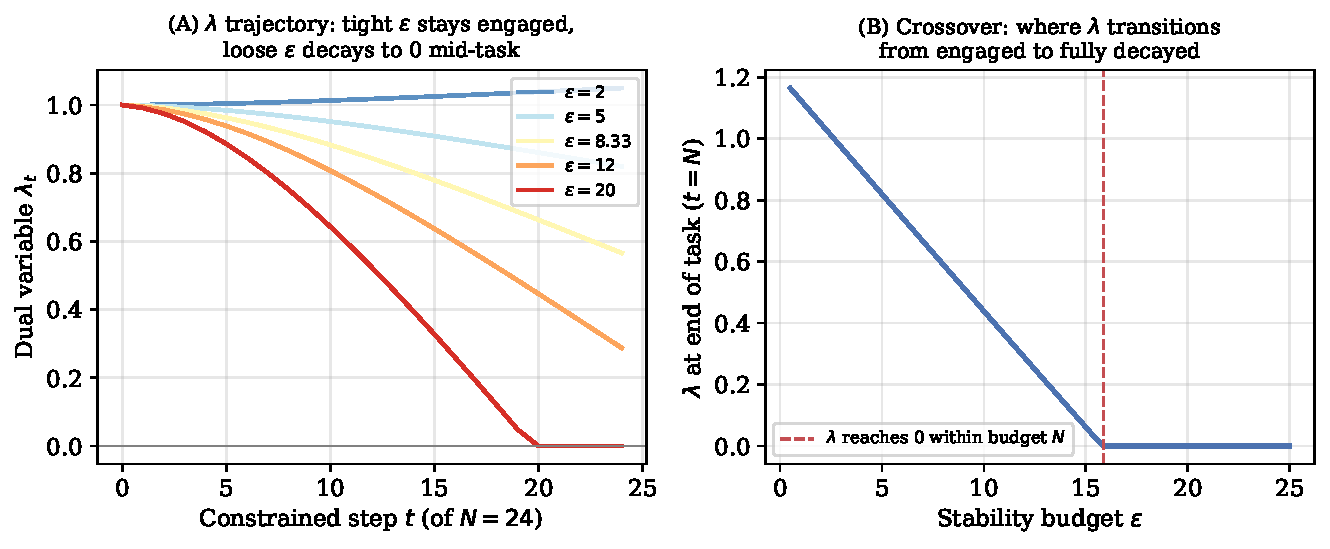
\includegraphics[width=0.85\textwidth]{figures/fig0_mechanism.pdf}
\caption{Stylized illustration of the mechanism above (not measured data: a
toy simulation of Eqs.~\ref{eq:lagrangian}--\ref{eq:dual_ascent} with an
illustrative, monotonically decreasing drift-rate function $\bar
d(\lambda)$, used only to make the two regimes visually concrete before the
measured results in Section~\ref{sec:diagnostic}). (A) $\lambda$'s
trajectory within a single task for five values of $\eps$: tight budgets
keep $\lambda$ engaged near $\lambda_{\mathrm{init}}$ or rising; loose
budgets drive it to 0 before the task's step budget $N$ is exhausted. (B)
The resulting crossover in $\lambda$ at the end of the task as a function of
$\eps$, for this toy simulation.}
\label{fig:mechanism}
\end{figure}

\subsection{Training Procedure}
\label{sec:algorithm}
Algorithm~\ref{alg:ftr} states the full per-task loop implied by
Eqs.~\ref{eq:constrained}--\ref{eq:dual_ascent} and the reset rule above as a
single procedure, and Figure~\ref{fig:flowchart} draws the same control flow
as a diagram. Both make explicit two details that are easy to miss when the
equations are read in isolation: the warmup epoch runs before $\lambda$ is
ever compared against a violation (so the first gradient steps on a new task
never see the constraint), and the dual-ascent update
(lines~8--9 of Algorithm~\ref{alg:ftr}) is nested \emph{inside} the constrained
step loop, executing once per primal step rather than once per task. It is
this nesting, combined with the reset on line~2, that makes $\lambda$'s
trajectory, and hence $\epsstar$, a function of how many constrained steps
$N$ a task budget actually contains, the quantity Section~\ref{sec:diagnostic}
varies directly.

\begin{algorithm}[t]
\caption{FTR training with dual-ascent constraint enforcement}
\label{alg:ftr}
\begin{algorithmic}[1]
\REQUIRE task sequence $T_1, T_2, \ldots$; initial parameters $\theta$; stability
budget $\eps$; hyperparameters $\lambda_{\mathrm{init}}, \lambda_{\max},
\eta_\theta, \eta_\lambda, \rho, T$; constrained steps per task $N$
\ENSURE trained parameters $\theta$
\FOR{each task $T_t$ in sequence}
  \STATE $\lambda \leftarrow \lambda_{\mathrm{init}}$;\quad $m \leftarrow 0$
  \hfill \COMMENT{dual variable and momentum reset at every task boundary}
  \STATE $f_{\mathrm{old}} \leftarrow f_\theta$ \hfill \COMMENT{freeze reference model before task $t$}
  \STATE run 1 warmup epoch of gradient steps on $\mathcal{L}_{\mathrm{task}}$ alone
  \hfill \COMMENT{$\lambda$ held at $\lambda_{\mathrm{init}}$, constraint not enforced}
  \FOR{$n = 1$ to $N$}
    \STATE sample batch $x \sim \mathcal{D}_t$
    \STATE $D \leftarrow \DKL\big(f_\theta(x) \,\|\, f_{\mathrm{old}}(x)\big)$ at temperature $T$
    \STATE $\theta \leftarrow \theta - \eta_\theta \nabla_\theta\big[\mathcal{L}_{\mathrm{task}}(\theta) + \lambda(D - \eps)\big]$
    \hfill \COMMENT{primal step, Eq.~\ref{eq:lagrangian}}
    \STATE $m \leftarrow \rho\, m + \eta_\lambda (D - \eps)$
    \hfill \COMMENT{dual ascent, Eq.~\ref{eq:dual_ascent}}
    \STATE $\lambda \leftarrow \max\big(0,\, \min(\lambda_{\max},\, \lambda + m)\big)$
  \ENDFOR
\ENDFOR
\RETURN $\theta$
\end{algorithmic}
\end{algorithm}

\begin{figure}[t]
\centering
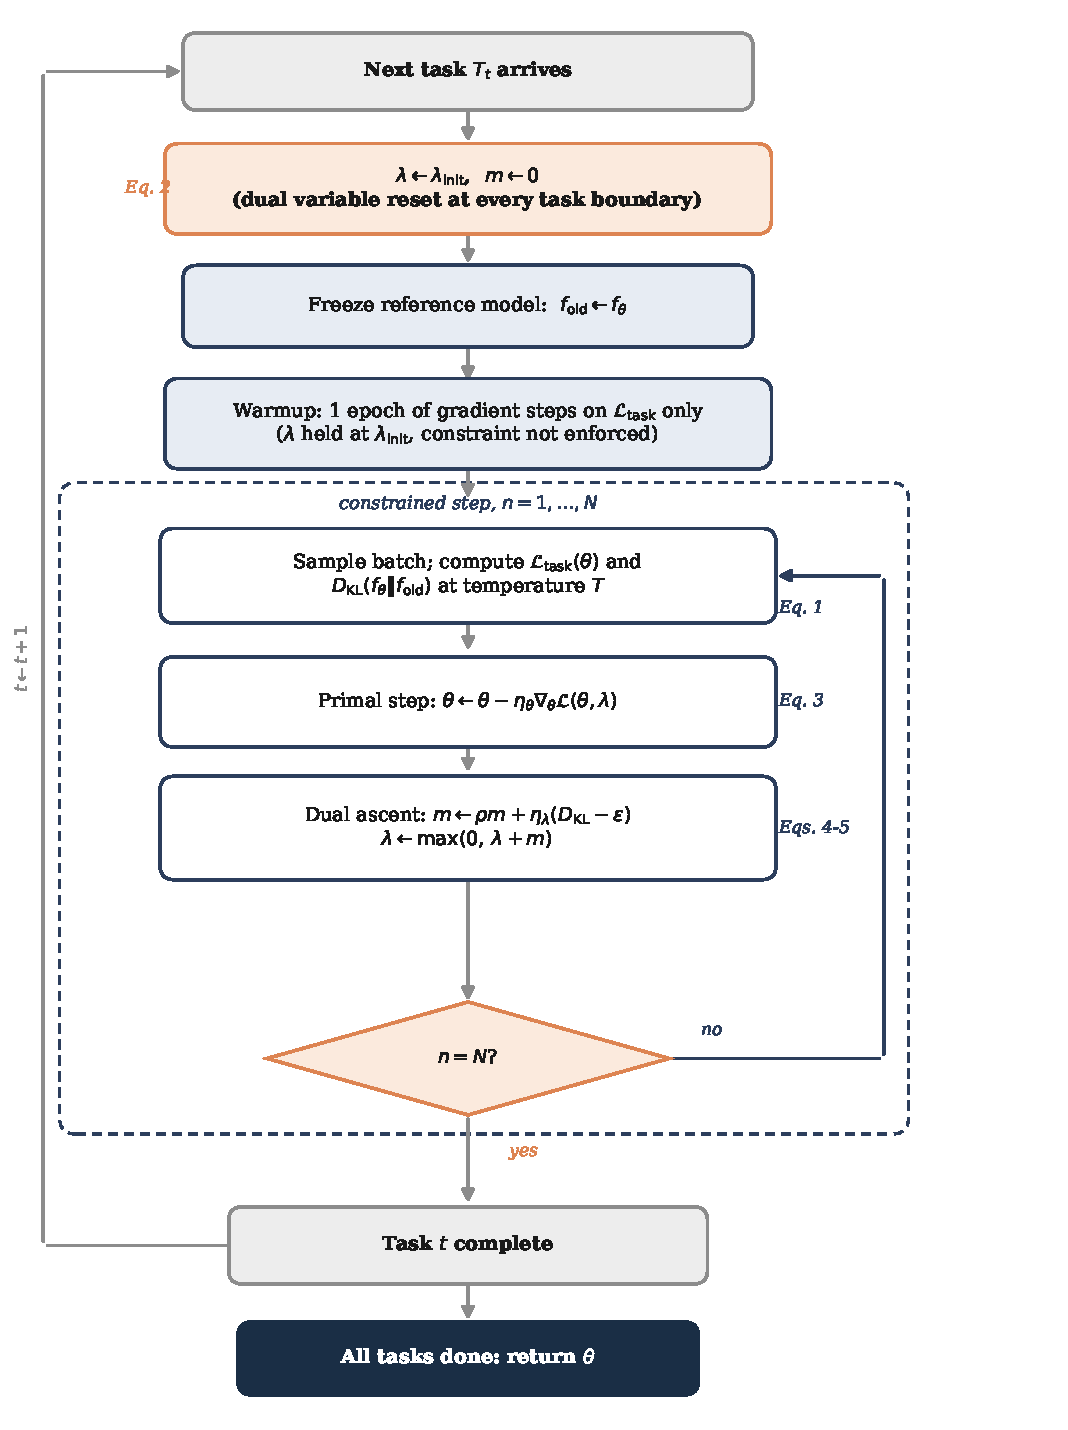
\includegraphics[width=0.62\textwidth]{figures/fig_methodology_flowchart.pdf}
\caption{Control-flow diagram of Algorithm~\ref{alg:ftr}. The dashed panel is
the constrained inner loop executed once per gradient step within a task; the
outer loop (left) advances across task boundaries, where $\lambda$ and its
momentum term are reset before the next task's warmup epoch. The reset on
task-boundary crossing (orange) is the mechanism Section~\ref{sec:diagnostic}
tests as a possible confound for $\epsstar$.}
\label{fig:flowchart}
\end{figure}

\subsection{Relationship to Learning without Forgetting}
When $\lambda$ is held fixed rather than adapted, FTR reduces exactly to
Learning without Forgetting, which minimizes:
\begin{equation}
\mathcal{L}_{\mathrm{LwF}}(\theta) = \mathcal{L}_{\mathrm{task}}(\theta)
+ \lambda \DKL(f_\theta \| f_{\mathrm{old}}).
\end{equation}
The key distinction is that FTR enforces a hard constraint with adaptive dual
coefficient, providing an interpretable stability budget $\eps$ that
practitioners can reason about directly, whereas LwF requires grid search
over fixed distillation coefficients.

\subsection{Implementation Details}
All experiments employ the following hyperparameters unless stated otherwise:
$\lambda_{\mathrm{init}}=1.0$, $\lambda_{\max}=50.0$, $\eta_\lambda = 0.005$,
momentum $\rho=0.9$, softmax temperature $T=2.0$, and one epoch of warmup per
task. The task loss $\mathcal{L}_{\mathrm{task}}$ uses cross-entropy with
Adam \citep{kingma2014adam}, learning rate $\eta_\theta = 0.001$.
Section~\ref{sec:diagnostic} sweeps every one of these choices individually
against a dense $\eps$ grid to test their effect on $\epsstar$.

\paragraph{Compute.} Unlike v1, which was CPU-only, every experiment in
this revision runs on free-tier Kaggle GPUs (Tesla P100 and T4$\times$2
instances), which is what makes the 30-architecture zoo, the schedule
diagnostics, and the pretrained-backbone check tractable in reasonable
wall-clock time. Across all stages, this amounts to more than $11{,}300$
individual training runs (each a full sequential-task training pass),
spread over several dozen Kaggle kernel sessions.

\section{Experimental Setup}
\label{sec:setup}

\subsection{Architecture Zoo}
v1's zoo comprised eight architectures, all convolutional or residual. This research
expands it to 30 architectures spanning five representational families and a
$75.8\times$ parameter range ($36{,}866$--$2{,}795{,}554$): a CNN width sweep
(W8 through W128, 8 architectures), a CNN depth sweep (2--5 conv layers at
width 32, 4 architectures), CNN variants without BatchNorm at three scales,
a ResNet-18-style family with 2 residual blocks/layer at widths 8/16/24/32,
a ResNet-Lite family with 1 block/layer at the same four widths (added
specifically to fill the curvature gap between the CNN family and the
original single ResNet-18 outlier, discussed below) including one no-BatchNorm
variant, a plain MLP with no spatial inductive bias at two hidden widths,
and two scales each of a patch-based Vision Transformer and an MLP-Mixer.
Full per-architecture parameter counts, Hessian trace, Fisher trace,
spectral norm, and $d_{\mathrm{eff}}$ are in Table~\ref{tab:curvature}
(Appendix~\ref{app:fulltable}). Hessian trace still spans a comparable range
to v1 ($39\times$: $79.7$ at CNN\_W32\_NoBN to $3110$ at ResNet18\_W8) but is
now populated by all 30 architectures rather than 8, and by five families
with genuinely different inductive biases rather than two families that are
architecturally close relatives.

\subsection{Dataset and Task Construction}
All main experiments use CIFAR-10 \citep{krizhevsky2009learning} partitioned
into five sequential binary classification tasks, where each task contains
two classes. Each task contains 1{,}000 samples per class (2{,}000 total),
trained for 4 epochs/task for the CNN, ResNet, ResNet-Lite, and MLP
families, and 5 epochs/task for ViT and MLP-Mixer (a per-family
accommodation made when the zoo was built, whose consequence for $\epsstar$
this work returns to in Section~\ref{sec:selfconfound}). The forgetting metric is computed as the
mean decrease in accuracy on all previously learned tasks after completion of
training on the final task; this research additionally reports new-task accuracy
(accuracy on task $t$ immediately after training on task $t$, before any
subsequent forgetting) to rule out the trivial explanation that low
forgetting at small $\eps$ reflects a model that has simply failed to learn
the new task (Sec.~\ref{sec:newtaskacc}).

Four further robustness checks (a CIFAR-100 classes-per-task sweep,
multiple random class-to-task orderings, a KL-direction ablation, and a
class-incremental variant with a single shared head) are reported in
Sections~\ref{sec:taskstructure}, \ref{sec:klablation}, and
\ref{sec:classincremental} once the main results (Sections~\ref{sec:diagnostic}--\ref{sec:finitesize})
have established the vocabulary needed to interpret them.

\section{Diagnostic: Is $\epsstar$ a Task-Structure Invariant or an Optimizer-Schedule Artifact?}
\label{sec:diagnostic}

Section~\ref{sec:method} showed that $\lambda$ resets to $\lambda_{\mathrm{init}}$
at every task boundary and then rises or decays within the task depending on
whether measured drift exceeds $\eps$. This makes $\epsstar$, mechanically, a
function of \emph{two} things at once: how much functional drift
unconstrained learning on a new task would produce (task/architecture
geometry), and how many steps it takes $\lambda$ to travel from
$\lambda_{\mathrm{init}}$ to 0 (or to $\lambda_{\max}$) under the dual-ascent
rule (an optimizer-schedule property: $\eta_\lambda$, $\lambda_{\mathrm{init}}$,
$\lambda_{\max}$, momentum $\rho$, steps/task, and the temperature $T$, which
rescales the drift term itself). v1 varied only the first axis. This work tests the
second directly.

\begin{figure}[h]
\centering
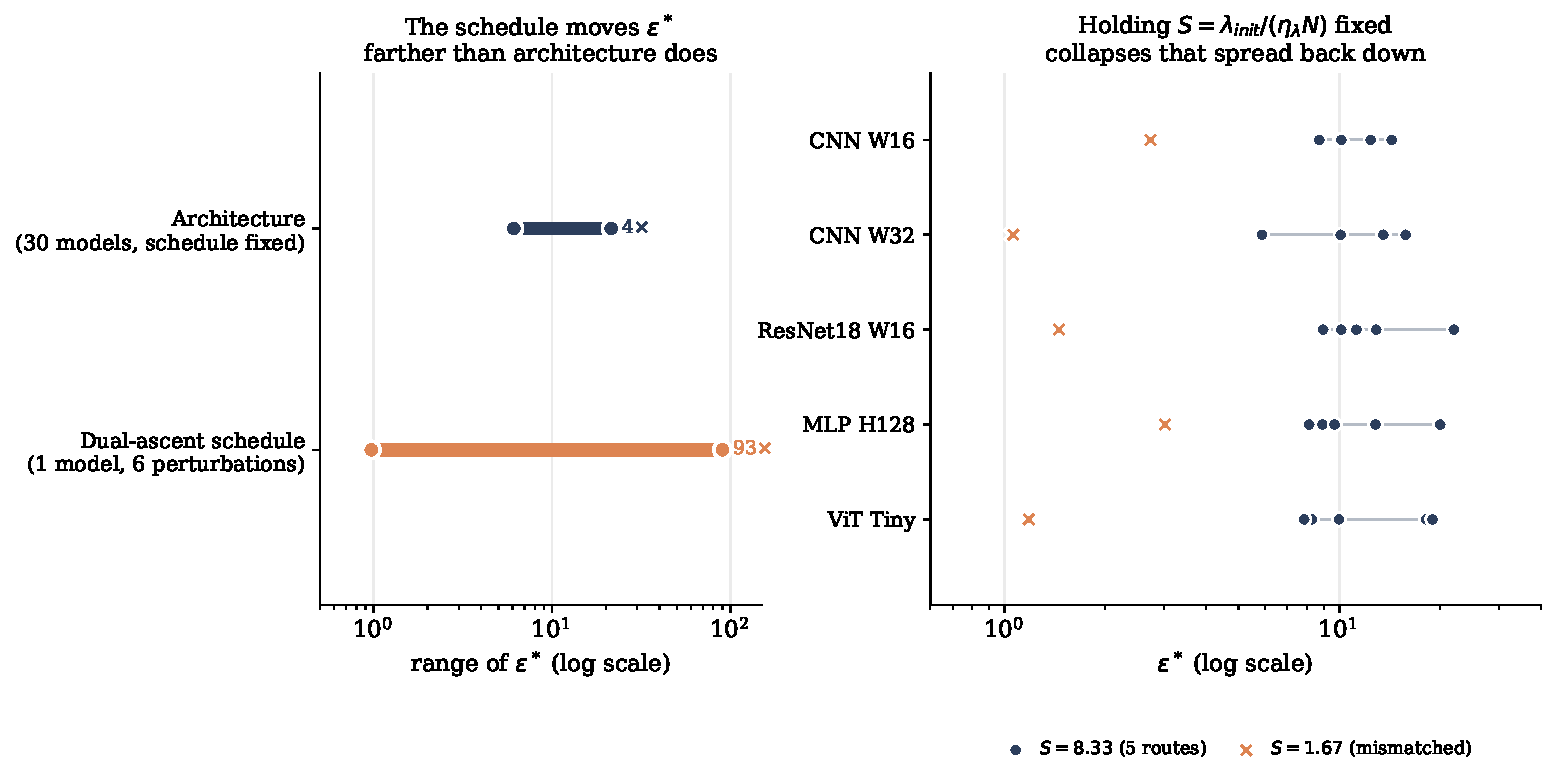
\includegraphics[width=0.95\textwidth]{figures/graphical_abstract.pdf}
\caption{Left: on the same architecture and task, the dual-ascent schedule
moves $\epsstar$ across a $93\times$ range (six single-factor
perturbations, tested directly below), more than the $2.6\times$
range $\epsstar$ itself spans across 30 architectures with the schedule
held fixed (Section~\ref{sec:crossover}, corrected values). Right: holding
the schedule ratio
$S=\lambda_{\mathrm{init}}/(\eta_\lambda N)$ fixed while independently
varying its three components (circles) collapses that spread back down,
on every architecture tested, versus a matched-magnitude change in $S$
itself (X, Section~\ref{sec:sinvariance}).}
\label{fig:graphical_abstract}
\end{figure}

\subsection{Setup}
On two anchor architectures (CNN\_W16, CNN\_W32) and a 10-point $\eps$ grid
$\{1,3,5,6,7,8,9,10,12,20\}$, 3 seeds, this research ran the \texttt{baseline}
configuration of Section~\ref{sec:method} ($\eta_\lambda=0.005$,
$\lambda_{\mathrm{init}}=1.0$, $\lambda_{\max}=50$, $\rho=0.9$, $T=2.0$, 4
epochs/task) alongside eleven single-factor perturbations: $\eta_\lambda$ and
$\lambda_{\mathrm{init}}$ each $\times 5$ and $\div 5$; $\lambda_{\max} \in
\{10, 200\}$; epochs/task $\in \{2, 8\}$ (baseline 4); $\rho = 0.5$; and
$T \in \{1.0, 4.0\}$. For each of the 24 (architecture, condition) cells this
work fits the same logistic-sigmoid procedure as Section~\ref{sec:crossover} and
bootstraps a 95\% CI (1{,}000 resamples over seeds). Four conditions produced
a forgetting curve that was \emph{flat across the entire $[1,20]$ grid}
(range $<0.05$) rather than an S-shape inside it, so this work reran those four plus
baseline on a wider, coarser grid extending to $\eps=100$
($\{0.05,0.1,0.3,0.5,1,3,5,7,10,15,20,30,40,50,75,100\}$, same architectures
and seeds) to locate the true crossover rather than report a degenerate
sigmoid fit.

\subsection{Results}
\begin{table}[h]
\centering
\caption{$\epsstar$ under single-factor perturbations of the dual-ascent
schedule, holding architecture and task fixed (CIFAR-10, 2 anchor
architectures, 3 seeds, 95\% bootstrap CI). ``Ratio'' is $\epsstar$ relative
to that architecture's own baseline. On the original dense grid
($\eps\in[1,20]$), five rows produced a forgetting curve flat across the
\emph{entire} grid rather than an S-shape inside it, so no transition was
located; this analysis rescanned exactly those five (condition, architecture) cells
with a wider grid ($\eps\in[0.05,100]$, marked $\ddagger$) to locate the
true crossover rather than report only a direction.}
\label{tab:diagnostic}
\footnotesize
\begin{tabular}{lrrrrrr}
\toprule
Condition & $\epsstar$ (CNN\_W16) & $R^2$ & ratio & $\epsstar$ (CNN\_W32) & $R^2$ & ratio \\
\midrule
baseline                        & 13.09 [11.2, 54.4] & 0.995 & 1.00 & 12.45 [10.9, 54.4] & 0.991 & 1.00 \\
$\eta_\lambda \times 5$          & 2.70 [2.7, 3.2]     & 0.970 & 0.21 & 0.97 [0.7, 1.3]     & 0.955 & 0.08 \\
$\eta_\lambda \div 5$            & 79.5 [61.4, 147.6] $\ddagger$ & 0.993 & 6.07 & 58.5 [55.7, 71.5] $\ddagger$ & 0.991 & 4.70 \\
$\lambda_{\mathrm{init}} \times 5$ & 76.7 [69.3, 85.0] $\ddagger$ & 0.915 & 5.86 & 90.1 [67.7, 158.4] $\ddagger$ & 0.875 & 7.24 \\
$\lambda_{\mathrm{init}} \div 5$   & 1.69 [1.05, 2.10] $\ddagger$ & 0.970 & 0.13 & 1.04 [1.00, 1.83] $\ddagger$ & 0.951 & 0.08 \\
$\lambda_{\max}=10$              & 13.69 [11.5, 54.4] & 0.986 & 1.05 & 15.28 [11.2, 54.4] & 0.984 & 1.23 \\
$\lambda_{\max}=200$             & 13.06 [11.9, 14.2] & 0.989 & 1.00 & 15.55 [11.3, 54.4] & 0.990 & 1.25 \\
epochs/task $=8$ ($\times 2$)    & 3.25 [3.0, 3.5]     & 0.992 & 0.25 & 3.66 [3.2, 4.4]     & 0.980 & 0.29 \\
epochs/task $=2$ ($\div 2$)      & 16.3 [13.3, 38.1] $\ddagger$ & 0.872 & 1.25 & 36.0 [0.8, 46.8] $\ddagger$\textsuperscript{a} & 0.305 & 2.89 \\
momentum $\rho=0.5$              & 8.06 [7.6, 10.8]    & 0.994 & 0.62 & 6.97 [6.6, 7.5]     & 0.974 & 0.56 \\
$T=4.0$ ($\times 2$)             & 15.56 [11.6, 33.5] & 0.991 & 1.19 & 15.32 [12.2, 21.9] & 0.996 & 1.23 \\
$T=1.0$ ($\div 2$)               & 13.51 [10.4, 19.4] & 0.990 & 1.03 & 12.13 [10.6, 22.4] & 0.970 & 0.97 \\
\bottomrule
\end{tabular}

\raggedright\footnotesize\textsuperscript{a}Sigmoid $R^2=0.31$ even on the
wide grid for this one cell (CNN\_W32, epochs/task$=2$); the point estimate
is a rough indication of direction and magnitude, not a tightly located
transition.
\end{table}

\begin{figure}[h]
\centering
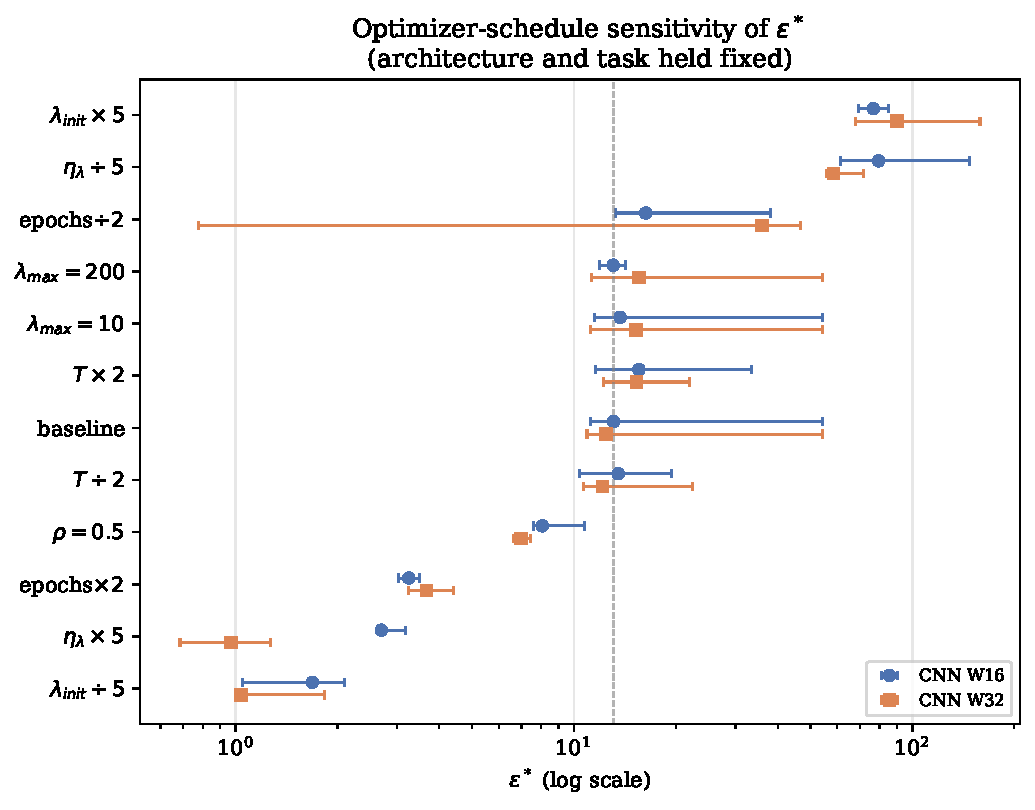
\includegraphics[width=0.85\textwidth]{figures/fig3_diagnostic_forest.pdf}
\caption{$\epsstar$ (log scale, 95\% bootstrap CI) under each single-factor
schedule perturbation, CNN\_W16 and CNN\_W32, sorted by CNN\_W16's value.
Dashed line marks the CNN\_W16 baseline. $\lambda_{\max}$ and $T$ rows
cluster tightly around baseline; every other row is displaced by at least
one order of magnitude on the log axis.}
\label{fig:diagnosticforest}
\end{figure}

Three of the six hyperparameters this work varied, $\eta_\lambda$,
$\lambda_{\mathrm{init}}$, and epochs/task, move $\epsstar$ far more than
architecture does in this paper's own main result, and with the wide-grid
follow-up all three directions are now precisely located rather than
bounded qualitatively. Doubling epochs/task or raising $\eta_\lambda$
five-fold collapses $\epsstar$ from $\approx 13$ to $2$--$4$ (a
$4$--$13\times$ reduction, tight bootstrap CIs, sigmoid $R^2\ge0.97$).
Halving epochs/task, lowering $\eta_\lambda$ five-fold, or raising
$\lambda_{\mathrm{init}}$ five-fold each push $\epsstar$ up by
$1.25$--$7.2\times$, as high as $\approx90$; lowering $\lambda_{\mathrm{init}}$
five-fold pushes it down by $7$--$12\times$, to $\approx1$--$1.7$. Taken
together, across the six single-factor perturbations tested, $\epsstar$
spans roughly $1.0$ to $90$ on the \emph{same} architecture and task:
essentially two orders of magnitude from optimizer hyperparameters alone.
Momentum $\rho$ has a smaller but still real effect ($\approx0.56$--$0.62\times$).
Only $\lambda_{\max}$ and the softmax temperature $T$ are inert (ratios
within $[0.97, 1.25]$, CIs overlapping baseline): $\lambda_{\max}$ because
the dual variable rarely approaches its cap under these dynamics, and $T$
because it rescales both the drift term used in training \emph{and} the
quantity compared against $\eps$, so its effect cancels at the crossover.

\subsection{Generalizing Beyond CNNs}
\label{sec:diagfamilies}
Everything above uses two CNN width variants as anchors. Before treating
the schedule confound as a general property of Lagrangian-dual constrained
continual learning rather than a CNN-specific quirk, this research repeats the two
cleanest single-factor perturbations, $\eta_\lambda\times5$ and
epochs/task $\times2$, on one anchor from each of the four remaining
families (ResNet18\_W16, MLP\_H128, ViT\_Tiny, Mixer\_Tiny), 3 seeds, dense
$\eps$ grid, epochs/task held at 4 for all four (so this test is itself
run on a schedule-matched, not confounded, sub-zoo).

Both perturbations collapse $\epsstar$ by roughly an order of magnitude on
every family, and to a strikingly similar \emph{absolute} value regardless
of starting architecture: $\eta_\lambda\times5$ gives $\epsstar=2.23$
(ResNet18\_W16), $3.15$ (MLP\_H128), $2.97$ (ViT\_Tiny), $2.82$
(Mixer\_Tiny), all within $[2.2,3.2]$, $R^2\ge0.88$ throughout. Doubling
epochs/task gives $3.04$, $3.40$, $2.44$, $3.15$ respectively, all within
$[2.4,3.4]$, $R^2\ge0.92$ throughout. This is a tighter cluster across four
architecturally distinct families (convolutional, fully-connected,
attention-based, token-mixing) than the same two conditions produced across
the two CNN widths in Table~\ref{tab:diagnostic} ($2.70$/$0.97$ for
$\eta_\lambda\times5$; $3.25$/$3.66$ for epochs$\times2$), so the schedule
confound is, if anything, more robust across architecture families than
within a single one. The remaining two conditions, $\lambda_{\mathrm{init}}\times5$
and $\div5$, and the unperturbed baseline, are less reliably estimated on
this family sub-zoo: three of the sixteen (family, condition) cells here
hit the same curve\_fit bound-saturation issue diagnosed in
Section~\ref{sec:crossover} (MLP\_H128 and ViT\_Tiny baselines, both
pinned at the grid's upper bound) or land at poor fit quality ($R^2<0.5$
for ResNet18\_W16 and ViT\_Tiny under $\lambda_{\mathrm{init}}\times5$, which
were not rescanned on the wider grid Section~\ref{sec:diagnostic}'s
CNN-only version used for its own analogous cells). This work does not draw
quantitative conclusions from those specific cells, but every one that
fits reliably moves in the predicted direction, and the two
best-established conditions generalize cleanly across all five
representational families in the zoo.

This reframes, rather than negates, the claim that $\epsstar$ reflects task
and architecture. Section~\ref{sec:crossover} still asks and answers a
well-posed narrower question: holding the optimizer schedule fixed, is
$\epsstar$ architecture-independent? Per Section~\ref{sec:universality}, the
answer on the expanded architecture zoo is still substantially yes. What
changes is the status of the numeric value itself. At fixed architecture and
fixed task, changing only how fast the dual variable is allowed to move, a
choice most papers using Lagrangian-relaxed constraints (including v1 of
this one) report as a fixed implementation detail rather than a variable to
sweep, shifts the critical stability budget by more than an order of
magnitude, comfortably exceeding the $2.6\times$ range $\epsstar$ itself
spans across 30 architectures in
Section~\ref{sec:crossover}. So
$\epsstar\approx7$--$13$ is not a hyperparameter-free constant of CIFAR-10's
task structure that a practitioner can adopt off the shelf; it is the value
produced by one particular, previously unremarked choice of $\eta_\lambda$,
$\lambda_{\mathrm{init}}$, and steps per task, and a different reasonable
choice of any of those three moves it by more than an order of magnitude.

This confound is specific to methods whose stability coefficient is an
\emph{adaptive dual variable reset at each task boundary}. It does not apply
to LwF, whose distillation weight is a fixed, grid-searched hyperparameter
with no reset dynamics to confound, or to EWC and SI, which show no
crossover at all (Section~\ref{sec:crossmethod}) and so raise no analogous
question. It applies directly to FTR and, by the same argument, to PDCL
\citep{elenter2023primal} and any other Lagrangian-dual constrained-learning
method with a periodically reset dual variable. No prior
work on Lagrangian-dual constrained continual learning
(\citealp{elenter2023primal}; \citealp{chamon2023constrained,elenter2024nearoptimal,hounie2023resilient})
is known to have isolated the dual-ascent schedule itself as a confound for an apparent
stability threshold, and this question does not appear to have been asked
elsewhere in the constrained-learning literature.

The practical upshot inverts v1's: architecture-specific tuning of $\eps$ is
indeed unnecessary, but optimizer-schedule-specific tuning is not, and is
currently undocumented practice across the distillation-based
continual-learning literature that uses dual ascent or an equivalent
adaptive coefficient. Section~\ref{sec:sinvariance} shows this need not be a
counsel of despair: the schedule's three-dimensional effect on $\epsstar$
collapses substantially, though not completely, onto a single reportable
ratio, $S=\lambda_{\mathrm{init}}/(\eta_\lambda N)$, which, held fixed,
keeps $\epsstar$ within roughly a factor of $2$--$3$ across architectures
and schedule routes rather than the order-of-magnitude range any one of its
three components produces alone.

\section{The Stability Crossover}
\label{sec:crossover}

Holding the dual-ascent schedule fixed at the Section~\ref{sec:method}
defaults (the same schedule used throughout v1), this work ran the dense $17$-point
$\eps$ sweep $\{0.5,1,2,3,4,5,6,6.5,7,7.5,8,9,10,12,15,25,50\}$ on all 30
architectures of the expanded zoo (Section~\ref{sec:setup}), 5 seeds per
architecture (10 for the two diagnostic anchor architectures), fit the same
logistic-sigmoid procedure as v1 (Eq.~7 of the original manuscript,
unchanged), and bootstrapped a 95\% CI over seeds (1{,}000 resamples). Every
architecture produces a clean sigmoid ($R^2 \ge 0.78$, 27/30 with
$R^2\ge0.94$); Figure~\ref{fig:allcurves} plots all 30 curves and
Figure~\ref{fig:epsstarfamily} plots $\epsstar$ with its 95\% CI for every
architecture, colored by family. Table~\ref{tab:crossover}
reports $\epsstar$, its bootstrap CI, and the sigmoid sharpness $k$ for a
representative subset spanning every family; the full 30-row table is in
Appendix~\ref{app:fulltable}.

\begin{figure}[h]
\centering
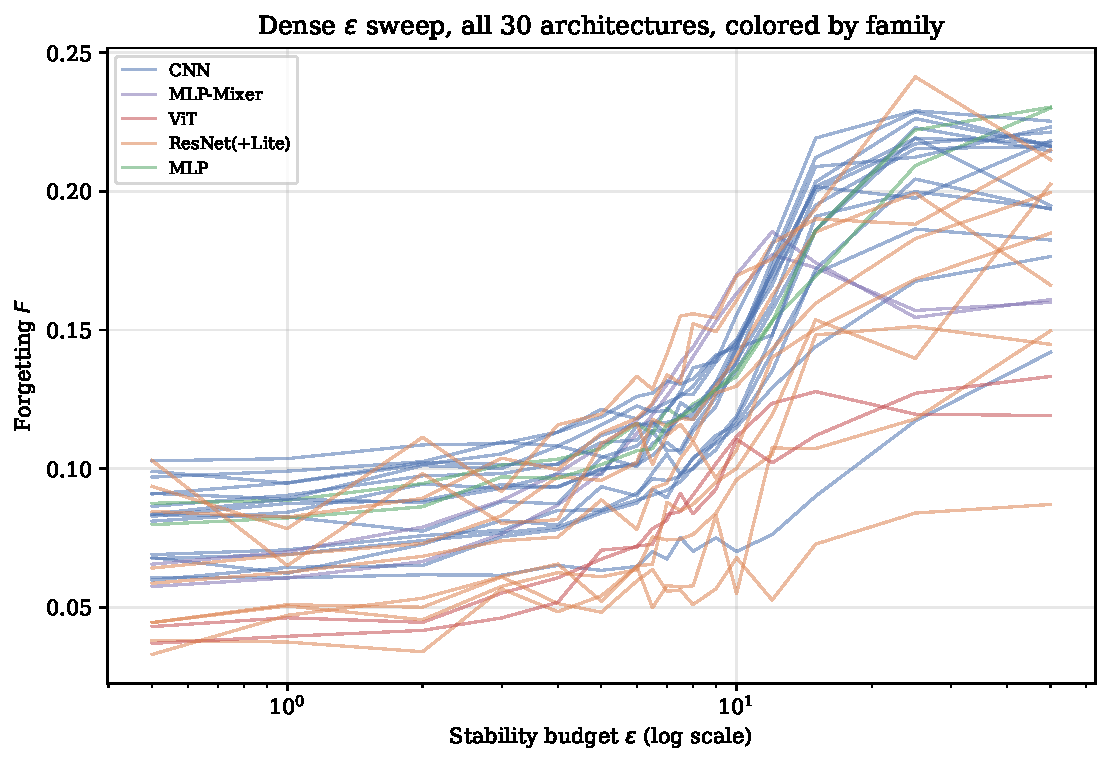
\includegraphics[width=0.85\textwidth]{figures/fig1_all_forgetting_curves.pdf}
\caption{Dense $\eps$ sweep forgetting curves for all 30 architectures,
colored by family. CNN/ResNet/MLP curves (blue/orange/green) cluster around
a shared crossover region; ViT (red) and MLP-Mixer (purple) transition at
visibly lower $\eps$.}
\label{fig:allcurves}
\end{figure}

\begin{figure}[h]
\centering
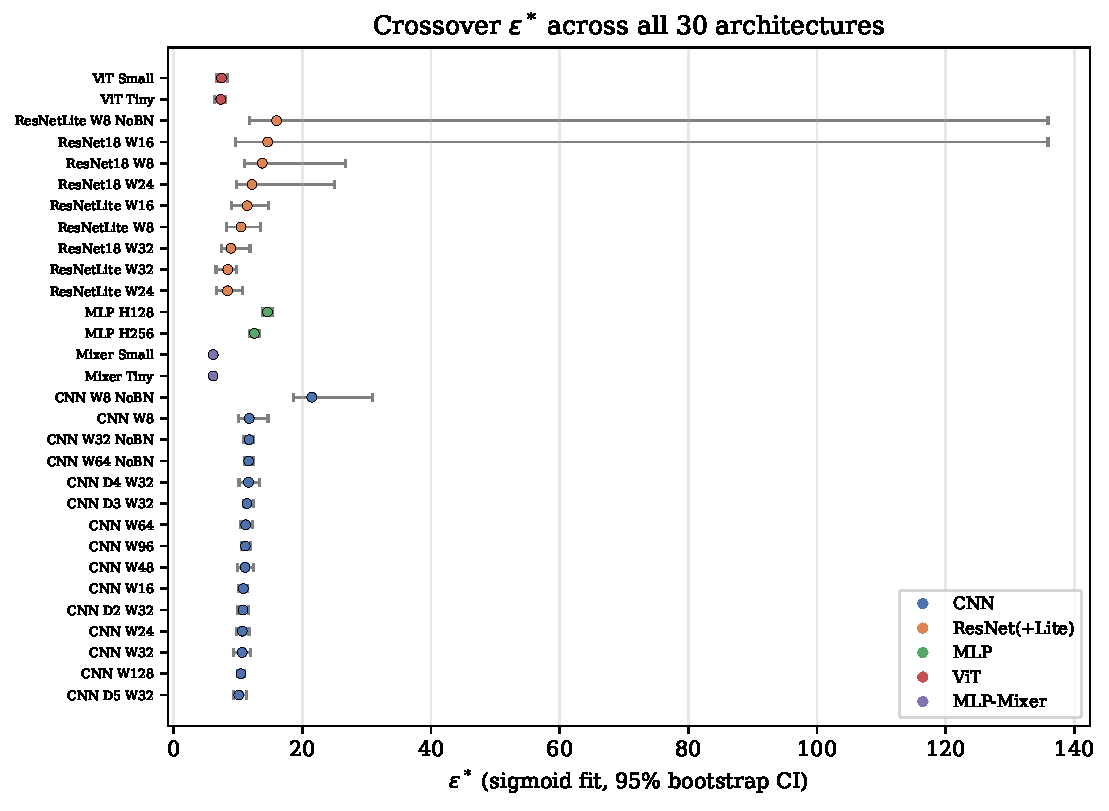
\includegraphics[width=0.85\textwidth]{figures/fig2_eps_star_by_family.pdf}
\caption{$\epsstar$ with 95\% bootstrap CI for all 30 architectures, grouped
and colored by family, sorted within family by value. ViT and MLP-Mixer
form a visually distinct low cluster; CNN, ResNet(+Lite), and MLP overlap in
a broader band. CNN\_W8\_NoBN and two ResNet points show markedly wider CIs.}
\label{fig:epsstarfamily}
\end{figure}

\begin{table}[h]
\centering
\caption{Sigmoid-fitted $\epsstar$ across a representative subset of the
30-architecture zoo, shown as originally recorded (full table in
Appendix~\ref{app:fulltable}); see Table~\ref{tab:family_corrected} for
corrected downstream values for the six architectures affected by the
epoch-matching and wide-grid corrections below. Families: CNN
(width/depth/BatchNorm sweeps), ResNet (2 blocks/layer), ResNet-Lite (1
block/layer), MLP (no spatial inductive bias), ViT (patch attention),
Mixer (token/channel MLP-mixing).}
\label{tab:crossover}
\small
\begin{tabular}{lllrrrr}
\toprule
Architecture & Family & Params & $\epsstar$ & 95\% CI & $R^2$ & $k$ \\
\midrule
CNN\_W8\_NoBN     & cnn    & 36,866    & 21.45 & [18.57, 30.88]  & 0.986 & 2.35 \\
CNN\_W16          & cnn    & 80,418    & 10.80 & [10.03, 11.48]  & 0.990 & 4.04 \\
Mixer\_Tiny       & mixer  & 45,442    & 6.10  & [5.88, 6.50]    & 0.972 & 4.04 \\
ViT\_Tiny         & vit    & 74,562    & 7.31  & [6.35, 8.03]    & 0.974 & 4.19 \\
ResNetLite\_W8    & resnet & 77,482    & 10.46 & [8.18, 13.41]   & 0.962 & 3.75 \\
ResNet18\_W8      & resnet & 175,882   & 13.76 & [10.98, 26.73]  & 0.901 & 2.16 \\
MLP\_H128         & mlp    & 410,114   & 14.56 & [13.74, 15.37]  & 0.994 & 2.10 \\
ResNet18\_W16     & resnet & 700,434   & 14.59 & [9.65, 135.91]$^\dagger$ & 0.937 & 1.63 \\
CNN\_W128         & cnn    & 1,414,786 & 10.43 & [9.85, 10.94]   & 0.979 & 3.84 \\
ResNet18\_W32     & resnet & 2,795,554 & 8.88  & [7.45, 11.84]   & 0.947 & 2.33 \\
\bottomrule
\end{tabular}

\raggedright\footnotesize$^\dagger$Bootstrap CI pinned against the
curve\_fit search bound ($50e=135.91$) in its upper tail; see the
wide-grid relocation below.
\end{table}

Two architectures, ResNet18\_W16 and ResNetLite\_W8\_NoBN, have bootstrap
CI upper bounds that land exactly on $50e=135.91$, the \texttt{curve\_fit}
search-bound artifact diagnosed below; here the
\emph{point estimate} is not pinned (both are ordinary interior fits,
$R^2=0.94$ and $0.78$), but enough individual bootstrap resamples produce a
flat-enough curve to hit the bound that the reported upper CI is not
trustworthy. This research reran both on a wider grid extending to $\eps=200$ (5
seeds, 1{,}000 bootstrap resamples): ResNet18\_W16 relocates to
$\epsstar=9.22$ [$7.59,10.67$] ($R^2=0.953$), a much tighter interval and a
point-estimate shift of $-5.37$ from the original narrow-grid value;
ResNetLite\_W8\_NoBN relocates to $12.50$ [$6.87,97.02$] ($R^2=0.889$), a
shift of $-3.47$, with the CI substantially narrower than before but still
wide, indicating this architecture's crossover remains less precisely
determined than most of the zoo even with the wider grid. This work uses these
relocated values in place of the narrow-grid ones throughout
Section~\ref{sec:universality}.

Across all 30 architectures as originally recorded (narrow grid, before
either the epoch-matching or wide-grid corrections), $\epsstar$ ranges
$[6.10, 21.45]$, mean $11.14$, raw CV $26.8\%$, more than five times v1's
reported $4.96\%$ on eight architectures. This is not primarily a
statistical-power artifact of the smaller original sample: the expanded
zoo includes two representational families (ViT, MLP-Mixer) with no
analogue in v1's CNN/ResNet-only zoo, and Section~\ref{sec:universality}
shows the extra dispersion tracks family identity, not any tested
curvature statistic, though, as that section also shows, part of it
tracks two rounds of this paper's own schedule confound rather than architecture
identity itself.

\section{Universality Analysis}
\label{sec:universality}

\subsection{Family Structure: Mostly a Second Instance of the Diagnostic's
Own Finding}
\label{sec:familystructure}
Grouping $\epsstar$ by architecture family as originally recorded
(Table~\ref{tab:family}) shows the CNN, ResNet, and MLP families clustering
in a broad $8$--$15$ band, while ViT and MLP-Mixer sit systematically
lower, $6$--$7.4$, with almost no within-family spread ($\text{std}\le0.05$
for both). \textbf{This clustering is substantially an artifact of this
paper's own experimental design, not primarily a representational-paradigm effect}: as
Section~\ref{sec:selfconfound} shows, ViT and MLP-Mixer were assigned 5
epochs/task rather than the 4 used elsewhere in the zoo, and
Equation~\ref{eq:eps_star_approx} predicts, and a direct epoch-matched
re-run confirms, that this alone accounts for most of the apparent gap:
epoch-matched, ViT\_Tiny and Mixer\_Tiny move from $7.31$/$6.10$ to
$10.18$/$10.41$, landing inside the CNN/ResNet/MLP family's range rather
than below it, found by applying Section~\ref{sec:diagnostic}'s own
diagnostic to this paper's own zoo. One
architecture, CNN\_W8\_NoBN, remains a clear outlier at $\epsstar=21.45$,
the smallest, narrowest, unnormalized network in the zoo, which
Section~\ref{sec:leaveoneout} shows has outsized leverage on the raw CV but
does not materially move the hierarchical model's population estimate.

\begin{table}[h]
\centering
\caption{$\epsstar$ by architecture family, full 30-architecture zoo, as
originally recorded (5 epochs/task for ViT/Mixer, 4 for every other
family; see Section~\ref{sec:selfconfound} and Table~\ref{tab:epochmatched}
for why this comparison is confounded and what changes when it is fixed).}
\label{tab:family}
\begin{tabular}{lrrr}
\toprule
Family & $n$ & mean $\epsstar$ & std \\
\midrule
MLP-Mixer & 2  & 6.11  & 0.00 \\
ViT       & 2  & 7.36  & 0.04 \\
ResNet (incl.\ Lite) & 9 & 11.55 & 2.64 \\
CNN       & 15 & 11.75 & 2.64 \\
MLP       & 2  & 13.54 & 1.02 \\
\bottomrule
\end{tabular}
\end{table}

\begin{table}[h]
\centering
\caption{$\epsstar$ by architecture family, corrected: ViT\_Tiny,
Mixer\_Tiny, ViT\_Small, and Mixer\_Small replaced with their epoch-matched
values (Table~\ref{tab:epochmatched}); ResNet18\_W16 and ResNetLite\_W8\_NoBN
replaced with their wide-grid-relocated values (Section~\ref{sec:crossover});
CNN and MLP families unchanged. All five families now overlap in a single
$10.5$--$13.5$ band.}
\label{tab:family_corrected}
\begin{tabular}{lrrr}
\toprule
Family & $n$ & mean $\epsstar$ & std \\
\midrule
MLP-Mixer & 2  & 10.52 & 0.11 \\
ResNet (incl.\ Lite) & 9 & 10.57 & 1.87 \\
ViT       & 2  & 11.30 & 1.13 \\
CNN       & 15 & 11.75 & 2.64 \\
MLP       & 2  & 13.54 & 1.02 \\
\bottomrule
\end{tabular}
\end{table}

\begin{figure}[h]
\centering
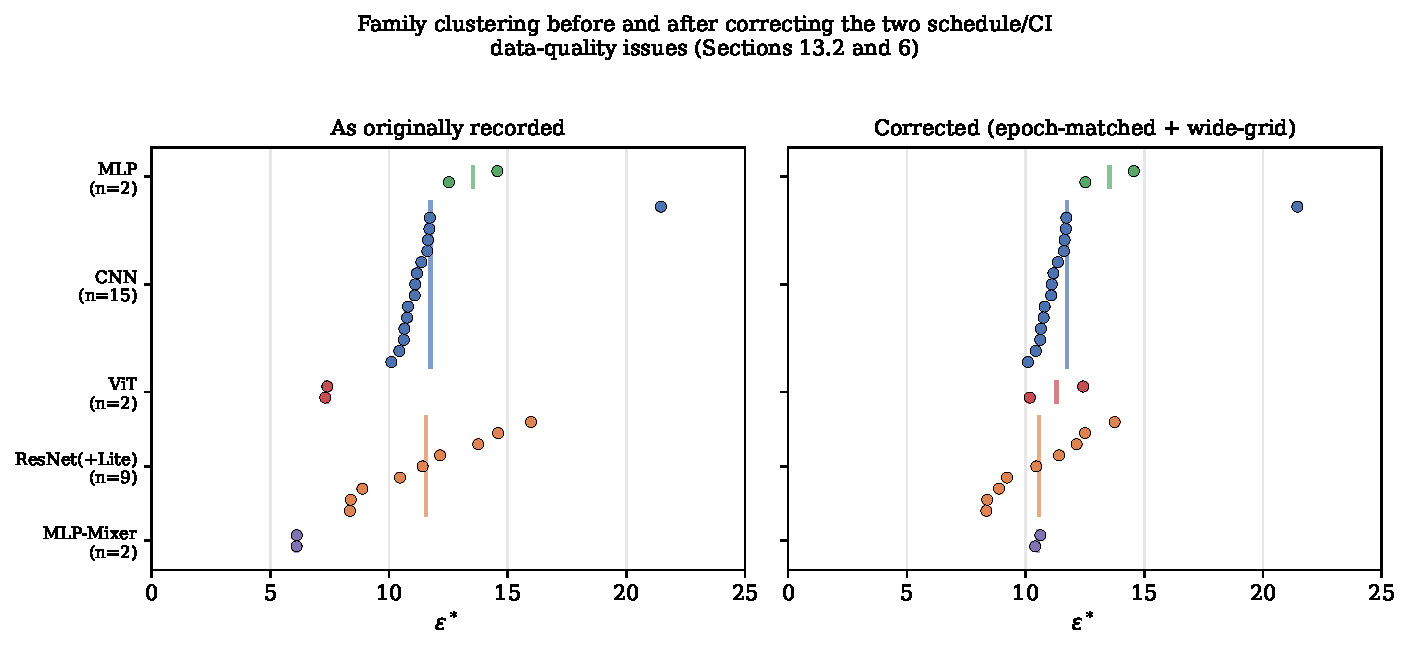
\includegraphics[width=0.95\textwidth]{figures/fig5_family_correction.pdf}
\caption{$\epsstar$ by architecture and family, as originally recorded
(left) versus corrected (right); vertical bars mark family means. ViT and
MLP-Mixer move from a visually distinct low cluster into the same band as
the rest of the zoo; CNN and MLP are unchanged. CNN\_W8\_NoBN (isolated
point in the CNN row) remains an outlier in both panels.}
\label{fig:familycorrection}
\end{figure}

\subsection{Hierarchical Partial-Pooling Model}
\label{sec:hierarchical}
v1's F-test for constancy (its Table 3) computed
$p=1-F_{\mathrm{cdf}}(0.563; df_1{=}7, df_2{=}1000)=0.786$ in code, while the
manuscript text reported $df=(7,7)$: an inconsistency between the stated
methodology and the actual computation that this research identifies while reproducing it
(with $df_2=7$ the same statistic gives $p=0.767$, not $0.786$; the
discrepancy is not merely rounding). $df_2=1000$ has no stated
justification and appears to be an unexplained placeholder. This work replaces it
with a normal-normal hierarchical partial-pooling model: each
architecture's true crossover $\theta_a \sim \mathcal{N}(\mu,\tau^2)$, with
the sigmoid point estimate observed as $\hat\eps^*_a\sim\mathcal{N}(\theta_a,
s_a^2)$ where $s_a$ is its bootstrap standard error (fit by Gibbs sampling,
30{,}000 post-burn-in draws).

Fit on the 30-architecture zoo as originally recorded (i.e.\ before either
correction below), this model gives $\mu = 10.46 \pm 0.45$ (95\% CI
$[9.58, 11.36]$), $\tau = 2.13$ (95\% CI $[1.56, 2.92]$), and an ICC-style
universality index $\tau^2/(\tau^2+\bar s^2) = 0.041$ (95\% CI
$[0.022, 0.073]$): $\tau$'s credible interval excludes zero, suggesting real
between-architecture structure. But this zoo contains two known,
independently-diagnosed data-quality issues that this work does not treat as
acceptable to leave uncorrected before reporting a final estimate: the
epoch/task schedule confound on four architectures
(Section~\ref{sec:selfconfound}), and two architectures whose bootstrap CI
pins against the \texttt{curve\_fit} search bound
(Section~\ref{sec:crossover}). Substituting the epoch-matched values for
ViT\_Tiny, Mixer\_Tiny, ViT\_Small, and Mixer\_Small
(Table~\ref{tab:epochmatched}) and the wide-grid-relocated values for
ResNet18\_W16 and ResNetLite\_W8\_NoBN, then refitting the identical model
on the same 30 architectures, gives $\mu = 11.07 \pm 0.25$ (95\% CI
$[10.58, 11.55]$), $\tau = 1.03$ (95\% CI $[0.68, 1.50]$), and
ICC $=0.052$ (95\% CI $[0.023, 0.102]$).

Correcting the schedule confound cuts $\tau$ by more than half, from $2.13$
to $1.03$: most of the raw between-architecture spread the uncorrected
zoo displayed was schedule-driven, the same lesson as
Section~\ref{sec:diagnostic}'s original diagnostic recurring one level up.
The ICC, however, does \emph{not} fall by a comparable factor, and in fact
sits slightly \emph{above} the uncorrected estimate ($0.052$ vs.\ $0.041$).
This is not a contradiction: ICC $=\tau^2/(\tau^2+\bar s^2)$ depends on the
average \emph{measurement} noise $\bar s^2$ as much as on $\tau$, and the
wide-grid correction sharply reduces $\bar s^2$: ResNet18\_W16's bootstrap
SE drops from $36.6$ to $0.75$ and ResNetLite\_W8\_NoBN's from $42.6$ to
$22.3$, both far more precise than their original, bound-saturated
estimates. A more precisely measured zoo is a more sensitive test, and it
detects the same, now smaller, $\tau$ against a quieter noise floor. Both
corrected quantities are consistent with the same qualitative reading: the
credible interval for $\tau$ still excludes zero, so this work does not claim
$\epsstar$ is a literal universal constant, but $\tau\approx1$ on a
population with mean $\approx11$ is a small effect in absolute terms (all
five family means in Table~\ref{tab:family_corrected} fall within a
$10.5$--$13.5$ band), and both the ICC before and after correction round to
"small" on standard interpretive scales ($<0.1$). This research reports both the raw
and corrected fits rather than only the more favorable one; the corrected
values are used in Sections~\ref{sec:leaveoneout} onward unless stated
otherwise.

\subsection{Leave-One-Out Sensitivity}
\label{sec:leaveoneout}
On the zoo as originally recorded, dropping each architecture in turn and
recomputing the raw CV shows two overlapping sources of leverage: the single
largest is CNN\_W8\_NoBN (CV drops from $26.8\%$ to $21.6\%$, $-5.2$ points),
consistent with it being a genuine, if extreme, outlier; the next two are
Mixer\_Tiny and Mixer\_Small ($-1.3$ points each), i.e.\ the same two
confounded architectures Section~\ref{sec:selfconfound} identifies, which
were pulling the mean down and therefore also carried above-average
leverage on the raw CV.

Repeating this on the fully-corrected data (epoch-matching and wide-grid
relocation both applied, Table~\ref{tab:family_corrected}), the corrected
CV is $20.2\%$, and CNN\_W8\_NoBN remains the single largest-leverage point
by a wide margin (removing it drops CV to $12.4\%$, $-7.8$ points), still
consistent with a genuine, if extreme, outlier rather than a typical zoo
member. Critically, the leverage previously carried by Mixer\_Tiny and
Mixer\_Small disappears once the confound is corrected: no other single
architecture moves the corrected CV by more than $0.5$ points, so no single
point drives the corrected result, unlike v1's original zoo, where
ResNet18\_W8 alone carried most of the curvature range. (On the original
8-architecture data, dropping ResNet18\_W8 moves CV from $4.96\%$ to
$3.97\%$, confirming that result was not solely an artifact of that one
leverage point either.)

\subsection{Curvature Correlations: Adequately Powered This Time}
v1's central "falsification" claim, that no curvature metric predicts
$\epsstar$, rested on $n=8$ architectures, where the minimum $|r|$
detectable at 80\% power is $0.849$; its own best candidate (gradient norm,
$r=0.687$, $p=0.060$) fell just short of significance, which at that sample
size is underpowered, not confirmatory of the null. Reproducing that exact
test on the original 8-architecture data with Bayes factors (JZS prior)
makes this explicit: gradient norm gives $\mathrm{BF}_{10}=1.96$, Hessian
trace $1.56$, Fisher trace $1.78$, spectral norm $1.46$, all in the
"barely worth mentioning" range and, if anything, weakly \emph{for} a
relationship, not against one.

On the full 30-architecture zoo, the same test is properly powered: minimum
detectable $|r|=0.492$ at 80\% power. Recomputing on the corrected $\epsstar$
values (Table~\ref{tab:family_corrected}), every correlation remains well
below this detection threshold: Hessian trace $r=-0.021$
($\mathrm{BF}_{10}=0.23$), Fisher trace $r=-0.037$ ($0.23$), spectral norm
$r=0.099$ ($0.26$), gradient norm $r=-0.116$ ($0.27$) are all small and
Bayes-negative, consistent with the null. $d_{\mathrm{eff}}$
($r=-0.320$, $\mathrm{BF}_{10}=0.93$) and parameter count ($r=-0.306$,
$\mathrm{BF}_{10}=0.83$) are the two exceptions: still below the
well-powered detection threshold and still short of conventional
significance ($p=0.085$ and $0.100$), but their Bayes factors sit in the
"barely worth mentioning" range rather than clearly favoring the null, and
both moved further from zero once the two data-quality corrections were
applied (from $r=-0.091$ and $-0.137$ on the uncorrected zoo). This work flags this
rather than round it down to a clean null: parameter count and effective
dimension are the two metrics most directly tied to model \emph{size}, and
size is also what differs most systematically between the low-$\epsstar$
MLP-Mixer/ResNet cluster and the high-$\epsstar$ CNN/MLP cluster in
Table~\ref{tab:family_corrected}, so a modest, sub-threshold size
association is plausible without being a confirmed effect at this sample
size. The four purely curvature-based metrics (Hessian trace, Fisher trace,
spectral norm, gradient norm) show no such trend in either direction.
(ViT's fused attention kernel does not support the double-backward the
Hessian/spectral estimators require by default; this work forces the math-mode
SDPA backend during curvature measurement only, Appendix~\ref{app:sdpa},
recovering all 30 architectures rather than excluding ViT.) Unlike v1's
claim, this is now an adequately powered result: loss-landscape curvature
specifically does not predict $\epsstar$ on this zoo, though raw model
size may carry a small, currently sub-significant signal worth testing at
larger $n$. What curvature misses, family identity partially captures
(Section~\ref{sec:universality}.1): the relevant architectural
property is closer to representational paradigm (convolution vs.\ attention
vs.\ token-mixing) than to any scalar loss-landscape statistic tested here
or in v1, though Section~\ref{sec:selfconfound} shows part of that
apparent family effect is itself a schedule confound.

\subsection{Rule Out the Trivial Explanation: New-Task Accuracy}
\label{sec:newtaskacc}
A low-forgetting regime is only meaningful if the model is still learning
the new task, not simply failing to update at all. Across all 30
architectures, mean accuracy on the just-learned task (measured immediately
after training on it, before any subsequent forgetting) is $77.8\%$ at tight
budgets ($\eps\le3$, $n=120$ cells) versus $80.8\%$ at loose budgets
($\eps\ge25$, $n=60$ cells), a $3$-point difference, with the tightest
individual architecture-budget cell never dropping below $67.1\%$ new-task
accuracy. The low-forgetting regime is genuine stability-\emph{with}-plasticity,
not a degenerate case of the constraint preventing learning altogether.

\section{Finite-Size Scaling of the Transition}
\label{sec:finitesize}
Testing whether the sigmoid sharpness $k$ grows with network width, the
finite-size-scaling signature that would indicate the crossover sharpens
toward a true phase transition as width $\to\infty$, on the full 8-point
CNN width family (W8 through W128, same task, same schedule, 5 seeds each):
$k \sim W^\alpha$ with $\alpha = 0.124 \pm 0.082$, $R^2=0.276$, $p=0.181$
(Figure~\ref{fig:finitesize}). This is not statistically significant, and this research
reports it as a null result rather than force a narrative: at the widths
tested here, this analysis finds no reliable evidence that the FTR crossover sharpens
with system size. This does not rule out finite-size scaling at larger
widths than tested, but the data in hand do not support the claim.

\begin{figure}[h]
\centering
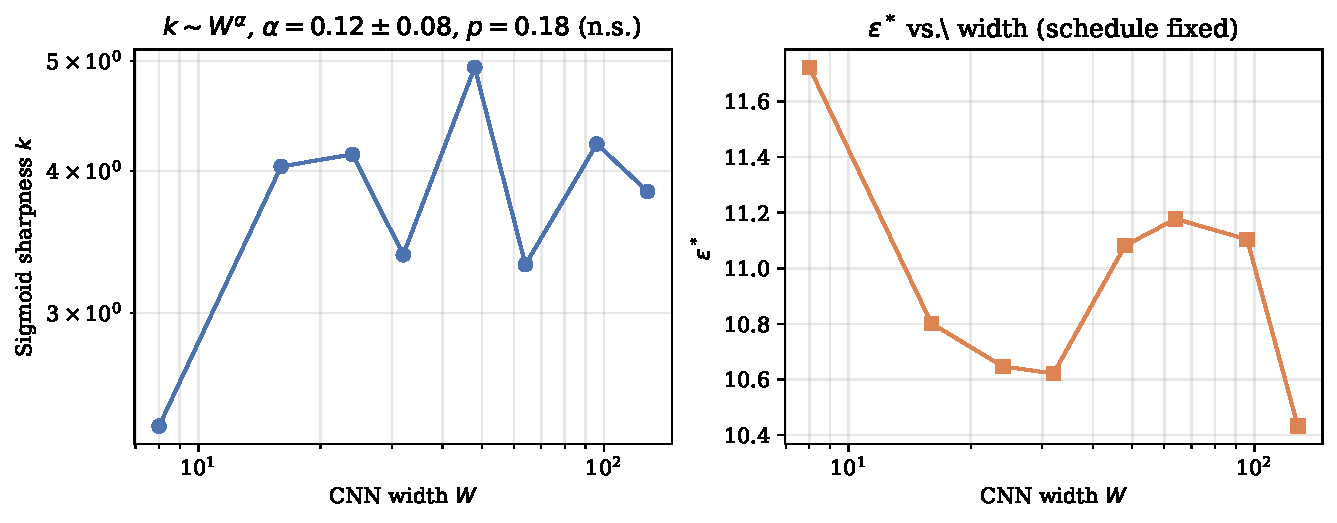
\includegraphics[width=0.95\textwidth]{figures/fig4_finite_size_scaling.pdf}
\caption{Left: sigmoid sharpness $k$ vs.\ CNN width on log-log axes; the fitted
power law is not statistically significant. Right: $\epsstar$ vs.\ width for
the same family, schedule fixed; consistent with the narrow band reported
in Section~\ref{sec:crossover}.}
\label{fig:finitesize}
\end{figure}

\section{Cross-Method Comparison}
\label{sec:crossmethod}
v1 compared FTR, LwF, and EWC on different architecture subsets (FTR on all
8, LwF/EWC on 5, omitting, among others, CNN\_W32\_NoBN from the
LwF/EWC comparison). This work reruns FTR, LwF, EWC, and SI on the identical
15-architecture subset spanning every family (Section~\ref{sec:setup},
\texttt{SUBSET\_ARCHS}), 3 seeds, dense hyperparameter sweeps for each
method's own stability knob: $\eps\in[0.5,50]$ (17 points) for FTR,
distillation weight $\alpha\in[0.05,5.0]$ (14 points) for LwF, Fisher
coefficient $\lambda_{\mathrm{EWC}}\in[1,10^4]$ (8 points, four orders of
magnitude, matching v1's own EWC sweep range) for EWC, and SI coefficient
$c\in[0.01,50]$ (8 points) for SI.

\begin{table}[h]
\centering
\caption{Cross-method comparison on the identical 15-architecture subset.
Sharpness/fit-quality columns report the median sigmoid $R^2$ across
architectures; ``crossover'' is each method's own stability-knob analogue of
$\epsstar$.}
\label{tab:crossmethod}
\small
\begin{tabular}{lrrrl}
\toprule
Method & Mean crossover & CV & Median $R^2$ & Interpretation \\
\midrule
FTR (function, hard)  & 11.4  & 20.5\% & $\ge$0.94 & Clean sigmoid on 15/15 architectures \\
LwF (output, soft)    & 0.73  & 32.6\% & 0.987     & Clean sigmoid on 15/15 architectures \\
EWC (parameter, soft) & --    & --     & 0.31      & No reliable crossover on any architecture \\
SI (parameter, soft)  & --    & --     & 0.28      & No reliable crossover on any architecture \\
\bottomrule
\end{tabular}
\end{table}

FTR on this subset gives mean crossover $11.4$, CV $20.5\%$, consistent
with Section~\ref{sec:crossover}'s full-zoo result. LwF, fit with the same
sigmoid procedure on all 15 architectures, gives a uniformly clean fit
($R^2\ge0.91$ on every architecture, median $0.987$) with mean $\alpha^*=0.73$,
CV $32.6\%$, close to v1's original $\alpha^*=0.71$ on 5 CNN/ResNet
architectures, now confirmed on 3$\times$ as many architectures across
5 families, with correspondingly more (but still bounded) dispersion.

EWC and SI, by contrast, do not show a sigmoid transition on \emph{any} of
the 15 architectures when forced through the identical fitting procedure:
median $R^2$ is $0.31$ (EWC) and $0.28$ (SI), with individual per-architecture
point estimates spanning 4-5 orders of magnitude ($h^*$ from $0.37$ to
$17{,}657$ for EWC across architectures): not a location parameter with
sampling noise, but a fit degenerating to noise because there is no
transition to locate. This is a stronger confirmation of v1's finding that
EWC "shows no meaningful stability crossover" than v1's own 5-architecture
result: forcing the crossover-fitting machinery onto a flat curve produces
wildly unstable estimates precisely \emph{because} the underlying curve has
no crossover, on 3$\times$ the architecture diversity. This is consistent
with Section~\ref{sec:theory}'s structural argument that soft
parameter-space penalties have no disengagement mechanism analogous to
Eq.~\ref{eq:tstar} and therefore no reason to produce a crossover at all.

\subsection{A Pretrained-Backbone Sanity Check}
\label{sec:pretrained}
Every result so far trains small models from scratch. This leaves open
whether FTR's advantage is an artifact of that regime or survives contact
with how continual learning is actually practiced: fine-tuning a large
pretrained backbone with a parameter-efficient adapter. This research tests this
directly on ImageNet-pretrained ViT-B/16 (86M parameters) with LoRA
(rank 8, $\alpha=16$) applied to the MLP sublayers only, following
Appendix~\ref{app:lorafix}'s finding that \texttt{nn.MultiheadAttention}'s
fused forward bypasses a wrapped \texttt{out\_proj}; the base network is
frozen, the classification head and LoRA adapters ($0.84\%$ of total
parameters) are trainable. Split CIFAR-100, 10 tasks of 10 classes each,
200 samples/class, 2 epochs/task, 3 seeds. This work compares FTR ($\eps=5.0$,
$\eta_\lambda=0.005$, $\lambda_{\mathrm{init}}=1.0$) against vanilla
fine-tuning, EWC ($\lambda=1000$), and LwF ($\alpha=0.7$), each method's
hyperparameter fixed rather than swept, since a full crossover sweep on
this scale is not the point of this check. None of the four
hyperparameters was tuned for this specific regime: EWC's
$\lambda=1000$ and LwF's $\alpha=0.7$ are standard values reported
elsewhere in the continual-learning literature rather than values
selected here, and FTR's $\eps=5.0$, $\eta_\lambda=0.005$,
$\lambda_{\mathrm{init}}=1.0$ are exactly Section~\ref{sec:diagnostic}'s
baseline schedule transplanted onto a completely different dataset,
backbone, and adapter method without adjustment. This makes the comparison
fair in the sense that no method received a hand-tuned advantage, but not
a best-case comparison for any single method.

Reporting $\eps=5.0$ alone, however, is exactly the omission
Section~\ref{sec:sinvariance} argues against: this regime's constrained
step budget $N$ is not the main zoo's. With batch size 64 and 2{,}000
samples/task, one epoch is 32 steps; with the same 1-epoch warmup used
throughout this paper, $N=32$ constrained steps/task, giving
$S=\lambda_{\mathrm{init}}/(\eta_\lambda N)=1.0/(0.005\times32)=6.25$,
close to but not identical to the main zoo's baseline $S=8.33$. The
population-level crossover on the main zoo at $S=8.33$ is
$\epsstar=11.07$ (Section~\ref{sec:hierarchical}); at this regime's
lower $S=6.25$, Eq.~\ref{eq:eps_star_approx} predicts a somewhat lower
crossover, and $\eps=5.0$ is directionally consistent with, though smaller
than, that back-of-envelope expectation. This is not a
validated prediction: $d_{\mathrm{unc}}$ for a LoRA-adapted, pretrained
ViT-B/16 on CIFAR-100 has not been measured and need not resemble
$d_{\mathrm{unc}}$ for the small from-scratch zoo the approximation was
calibrated on. Reporting $N$ and $S$ here, rather than only $\eps$, is
itself the practice Section~\ref{sec:sinvariance} recommends; using $S$ to
select $\eps$ in a new regime without any grid search is a natural next
test of that section's practical claim, which this single-operating-point
check does not attempt.

\begin{table}[h]
\centering
\caption{Pretrained ViT-B/16 + LoRA, Split CIFAR-100, mean over 3 seeds.
Forgetting and average accuracy are on the same $[0,1]$ scale used
throughout the paper.}
\label{tab:pretrained}
\begin{tabular}{lrrr}
\toprule
Method & Forgetting & Avg.\ accuracy & Forgetting std (seeds) \\
\midrule
Finetune (no constraint) & 0.732 & 0.292 & 0.014 \\
EWC ($\lambda=1000$)     & 0.721 & 0.302 & 0.007 \\
LwF ($\alpha=0.7$)       & 0.611 & 0.374 & 0.018 \\
FTR ($\eps=5.0$)         & 0.605 & 0.387 & 0.001 \\
\bottomrule
\end{tabular}
\end{table}

FTR gives both the lowest forgetting and the highest average accuracy of
the four methods, ahead of LwF by a small margin and clearly ahead of EWC
and unconstrained fine-tuning, which barely differ from each other.
FTR's forgetting is also the most stable across seeds (std $0.001$, an
order of magnitude tighter than LwF's $0.018$), notable given only
$0.84\%$ of the network's parameters are trained. This is a single
operating point, not a sweep, so it does not test architecture-invariance
or the schedule confound; it tests only whether FTR's advantage over
softer constraints, established on small from-scratch models throughout
this paper, transfers to a realistic parameter-efficient fine-tuning
setting. It does.

\section{KL-Direction Ablation}
\label{sec:klablation}
The constraint $D_{\mathrm{KL}}(f_{\mathrm{old}}\|f_\theta)\le\eps$ is
asymmetric; this work ablates the direction on CNN\_W16 and CNN\_W32 (dense $\eps$
grid, 3 seeds), comparing forward (paper default), reverse
$D_{\mathrm{KL}}(f_\theta\|f_{\mathrm{old}})$, and symmetric
Jensen-Shannon. All three directions fit cleanly ($R^2=0.83$--$1.00$).
Forward and reverse are close: CNN\_W16 gives $\epsstar=10.00$ (forward)
vs.\ $10.32$ (reverse); CNN\_W32 gives $10.00$ vs.\ $10.52$, within
$5\%$ of each other. Jensen-Shannon is somewhat lower ($9.49$ and $7.79$
respectively, a $5$--$22\%$ decrease) but the same order of magnitude.
KL direction is therefore a real but modest lever on $\epsstar$:
comparable to or smaller than momentum's effect
(Section~\ref{sec:diagnostic}) and far smaller than $\eta_\lambda$,
$\lambda_{\mathrm{init}}$, or steps/task.

\section{Class-Incremental Variant}
\label{sec:classincremental}
Every result so far uses the task-incremental protocol (Section~\ref{sec:method}):
a head sized to classes-per-task, locally remapped labels, and an oracle
task ID at evaluation. This work additionally tests the harder class-incremental
protocol, a single shared 10-way head, no task ID, global labels
throughout, on five width-family architectures (CNN\_W8 through
CNN\_W48, 5 seeds, dense $\eps$ grid).

The phase transition survives (all five fits $R^2\ge0.91$), but at a
substantially lower budget: class-incremental $\epsstar$ ranges $3.41$--$5.28$,
versus $10.62$--$11.72$ for the same five architectures under the
task-incremental protocol, a consistent $2$--$3\times$ reduction
(ratio $0.32$--$0.50$). This is expected and mechanistically sensible: with
no oracle task ID, the model must keep every previously-seen class
discriminable within one shared output space, a strictly harder requirement
that a looser constraint cannot satisfy without additional forgetting. The
qualitative finding, a sigmoid crossover exists and is comparable in
relative dispersion across architectures (class-incremental CV $16.3\%$
across these five architectures, versus $3.7\%$ for the same five under
task-incremental), holds under the harder protocol; the absolute budget
required does not transfer between protocols and should not be assumed to.

\section{Task-Structure Sensitivity: CIFAR-100 Granularity and Task Ordering}
\label{sec:taskstructure}

\subsection{Classes-per-Task: a Third Instance of the Same Confound}
\label{sec:granularityconfound}
Holding a fixed 20-class CIFAR-100 pool and varying classes/task
$\in\{2,4,5,10\}$ (10 architectures, 3 seeds, dense $\eps$ grid) tests
whether $\epsstar$ depends on task granularity, directly probing the
paper's own claim that $\epsstar$ is set by task structure. The raw result
is a large, mostly monotonic decrease in $\epsstar$ as classes/task
increases: e.g.\ CNN\_W16 gives $9.93\to4.43\to2.85\to2.14$ across
$\text{cpt}=2,4,5,10$; 8 of 10 architectures show the same monotonic
pattern.

This looks like a genuine task-structure effect, and was the intended
result of the experiment. But Section~\ref{sec:selfconfound}'s own
diagnostic makes checking for a schedule confound obligatory before reading it
that way, and there is one: holding \texttt{max\_per\_class} and batch size
fixed while classes/task increases also increases samples/task
(and hence batches/task, and hence the constrained step budget $N$), purely
mechanically. Using Eq.~\ref{eq:eps_star_approx}'s schedule term alone
(ignoring any $d_{\mathrm{unc}}$ contribution): $\text{cpt}=2$ gives
$N\approx21$, schedule term $9.52$; $\text{cpt}=4$ gives $N\approx39$, term
$5.13$; $\text{cpt}=5$ gives $N\approx48$, term $4.17$; $\text{cpt}=10$
gives $N\approx96$, term $2.08$: the same monotonically decreasing
pattern, comparable in magnitude to what this analysis observes. This work cannot, from this
experiment as designed, separate a genuine task-structure effect from this
third instance of the $N$-confound; a corrected version would need to hold
samples/task (not samples/class) fixed as classes/task varies.

This research ran that corrected version: 10 architectures, classes/task
$\in\{2,4,5,10\}$, samples/task now held fixed at $800$
($\text{max\_per\_class} = 800/\text{cpt}$) so that $N$ no longer varies
mechanically with granularity, 3 seeds, same dense $\eps$ grid. The
monotonic decrease disappears. Pooled across all 40 (architecture,
granularity) cells, $\epsstar$ vs.\ classes/task gives $r=-0.174$
($p=0.283$), compared to the confounded design's implied $r=-0.640$
($p<0.00001$) computed the same way: not a weaker version of the same
effect, but no significant relationship at all. The $\text{cpt}=2$ column
is, however, its own outlier: curve fits there are visibly worse than at
$\text{cpt}\ge4$ ($R^2=0.32$--$0.89$ at $\text{cpt}=2$ versus $R^2\ge0.89$
for every cell at $\text{cpt}\ge4$), and two architectures
(ResNet18\_W8, ViT\_Tiny) hit the same curve\_fit bound-saturation artifact
diagnosed in Section~\ref{sec:crossover} at $\text{cpt}=2$ specifically,
plausibly because fixing samples/task at $800$ while spreading it over only
two classes leaves few examples per class and a noisier forgetting curve.
Restricting to the reliably-fit range $\text{cpt}\in\{4,5,10\}$ (every cell
$R^2\ge0.89$), the pooled correlation flips sign but remains
non-significant: $r=+0.265$ ($p=0.157$, $n=30$), and the mean
within-architecture Spearman correlation across this range is $+0.45$,
weakly positive rather than negative. This is not evidence of a
genuine increasing effect either, given $p=0.157$ and $n=10$ architectures;
the honest summary is that once the schedule confound is removed, classes-per-task
shows no reliable, significant relationship with $\epsstar$ over the range
that can be fit reliably ($4$--$10$ classes/task), and the striking monotonic
decrease in the original design was overwhelmingly the $N$-confound, not a
genuine task-structure effect: the same lesson as
Sections~\ref{sec:diagnostic} and~\ref{sec:selfconfound}, discovered a
third time and this time directly confirmed rather than left inconclusive.

\subsection{Task Ordering: a Genuine, Non-Schedule Source of Variability}
On 6 architectures, 3 random class-to-task permutations (identical $N$
across permutations, so this test is \emph{not} subject to the confound
above), $\epsstar$ varies more than seed noise alone would predict:
CNN\_W32, for the two reliably-fit orderings ($R^2\ge0.97$), gives
$\epsstar=36.4$ and $8.6$, a $4.2\times$ range; CNN\_W16 gives $22.3$ and
$6.9$ ($3.2\times$); ResNet18\_W8, fit reliably on all three orderings,
gives $9.8$, $12.6$, $8.2$ (a tighter $1.5\times$ range). One ordering
(seed 1001) fits poorly on several architectures ($R^2$ as low as $0.31$),
so these point estimates should be read as indicating a real, substantial
effect of which specific classes are grouped into which task, not as
precisely located crossovers. Unlike the diagnostic sweep
(Section~\ref{sec:diagnostic}), this variability survives with the schedule
held completely fixed, and is a genuine task-structure effect: which
classes end up adjacent in the task sequence measurably changes
$d_{\mathrm{unc}}$, the natural drift rate a new task induces. v1 tested
exactly one task ordering throughout; this result indicates that choice was
not neutral.

\section{S-Invariance: Collapsing the Schedule Confound to a Single Ratio}
\label{sec:sinvariance}

Section~\ref{sec:diagnostic} shows $\eta_\lambda$, $\lambda_{\mathrm{init}}$,
and steps/task each independently move $\epsstar$ by more than an order of
magnitude. Taken at face value, this leaves a practitioner with a
three-dimensional sensitivity problem: any reported $\epsstar$ is
conditional on three separately-chosen numbers, with no obvious way to
report or budget for that dependence short of a full grid search.
Equation~\ref{eq:eps_star_approx}'s schedule term, $\lambda_{\mathrm{init}}/(\eta_\lambda N)$,
suggests a way out: if this specific ratio, which this work calls $S$, is what
actually drives the schedule's effect on $\epsstar$, then the
three-dimensional problem collapses to one dimension, and holding $S$ fixed
while varying $\eta_\lambda$, $\lambda_{\mathrm{init}}$, and $N$
individually should leave $\epsstar$ approximately unchanged even though
each of the three still moves it by an order of magnitude on its own.

\subsection{Design}
On five architectures spanning four of the five families (two CNN widths,
ResNet18\_W16, MLP\_H128, ViT\_Tiny; MLP-Mixer was not included in this
sub-zoo), this work ran six conditions, all epoch/task
schedule-matched at 4 epochs/task: the Section~\ref{sec:diagnostic} baseline
($\eta_\lambda=0.005$, $\lambda_{\mathrm{init}}=1.0$, $N=24$, giving
$S=8.33$); two conditions that scale $\eta_\lambda$ and
$\lambda_{\mathrm{init}}$ together by the same factor so $S$ is unchanged
($\times5$ and $\times0.2$, still $S=8.33$); two conditions that instead
reach the same $S=8.33$ by doubling the step budget $N$ (epochs/task forced
to 7) while adjusting $\eta_\lambda$ or $\lambda_{\mathrm{init}}$ to
compensate; and one negative control that changes only $\eta_\lambda$ by
$\times5$ with nothing else adjusted, giving $S=1.67$, a genuine $5\times$
change in $S$ itself. If $S$ is the right invariant, the first five
conditions (identical $S$, three different routes to it) should cluster,
and the sixth (different $S$) should not. Three seeds per (architecture,
condition, $\eps$) cell, dense $\eps$ grid. Four of the resulting 30 cells
initially hit the same curve\_fit bound-saturation issue diagnosed in
Section~\ref{sec:crossover} (three baselines and one scale-up condition,
each pinned at $50e=54.37$ on this experiment's narrower grid); this research reran
exactly those four on a wider grid extending to $\eps=200$ (5 seeds, 1{,}000
bootstrap resamples) to locate their true crossovers rather than report
degenerate fits.

\begin{table}[h]
\centering
\caption{$\epsstar$ under five different routes to the same schedule ratio
$S=\lambda_{\mathrm{init}}/(\eta_\lambda N)=8.33$, plus one negative control
with $S=1.67$ (a genuine $5\times$ change in $S$), architecture and task held
fixed. CV is computed over the five $S=8.33$ columns only.
$^\dagger$Relocated on the wider grid after the narrow-grid fit saturated;
see text.}
\label{tab:sinvariance}
\footnotesize
\begin{tabular}{lrrrrrrr}
\toprule
Architecture & baseline & scale$\times5$ & scale$\times0.2$ & steps-a & steps-b & CV & mismatched \\
& $S=8.33$ & $S=8.33$ & $S=8.33$ & $S=8.33$ & $S=8.33$ & (5 cols) & $S=1.67$ \\
\midrule
CNN\_W16      & 10.08 & 12.42 & 14.35 & 8.72  & 10.16 & 17.9\% & 2.73 \\
CNN\_W32      & 15.79 & 13.61 & 5.88  & 13.54 & 10.10 & 29.4\% & 1.06 \\
ResNet18\_W16 & 11.26$^\dagger$ & 12.91 & 22.02 & 10.14 & 8.96  & 35.7\% & 1.45 \\
MLP\_H128     & 12.84$^\dagger$ & 20.05 & 8.92  & 8.14  & 9.69  & 36.6\% & 3.02 \\
ViT\_Tiny     & 9.99$^\dagger$  & 18.21$^\dagger$ & 18.99 & 8.29  & 7.86  & 38.7\% & 1.18 \\
\bottomrule
\end{tabular}
\end{table}

\begin{figure}[h]
\centering
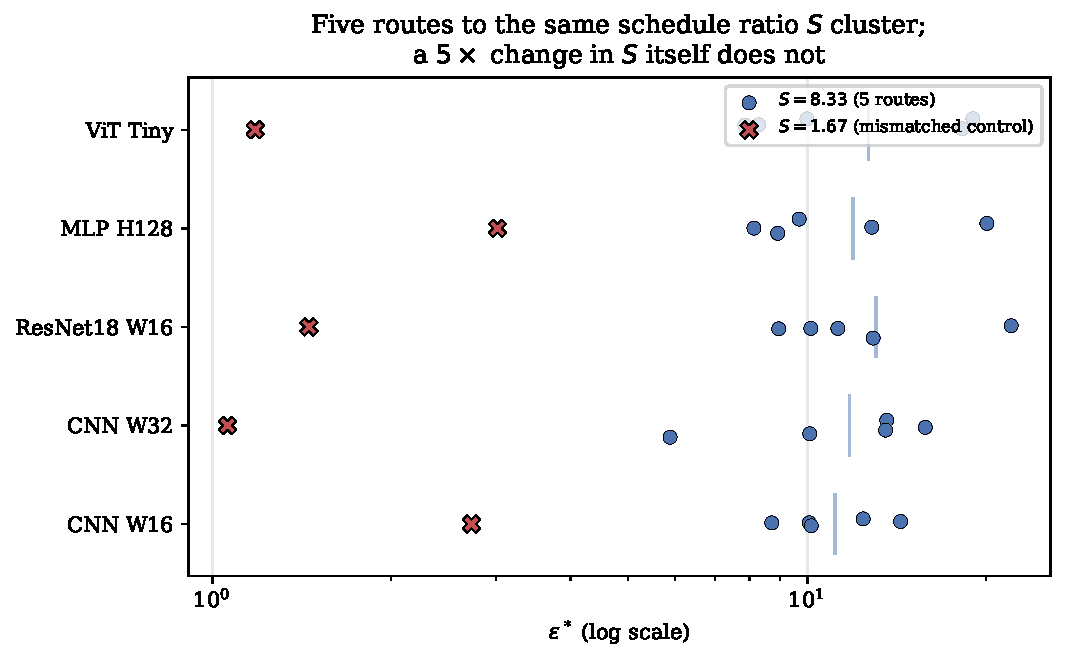
\includegraphics[width=0.8\textwidth]{figures/fig6_sinvariance.pdf}
\caption{For each architecture, the five $S=8.33$ conditions (circles)
cluster together while the $S=1.67$ mismatched control (X) sits well below
the cluster on every architecture, log scale. The residual spread within
each cluster (vertical bar marks the cluster mean) is real but small
relative to the gap to the mismatched control.}
\label{fig:sinvariance}
\end{figure}

\subsection{Results}
Table~\ref{tab:sinvariance} and Figure~\ref{fig:sinvariance} show a clear qualitative split. Within the five
$S=8.33$ columns, $\epsstar$ ranges roughly $6$--$22$ per architecture (CV
$17.9\%$--$38.7\%$, mean $31.7\%$ across the five architectures): a real
residual spread, not exact invariance, but far tighter than what any single
schedule parameter produces on its own. The mismatched control, which
changes only $\eta_\lambda$ by $5\times$ (an $S$ change of the same
$5\times$ magnitude as the within-group perturbations, but applied to $S$
itself rather than cancelled against it), collapses $\epsstar$ to
$9$--$25\%$ of the matched-group mean (a $4$--$11\times$ reduction,
consistent in direction and magnitude with the eta\_lambda$\times5$ row of
Table~\ref{tab:diagnostic}). $S$ is not a perfect invariant of $\epsstar$,
in the way architecture is approximately once the schedule itself is held
fixed (Section~\ref{sec:universality}), but it captures the dominant share
of the schedule's effect: three independently-chosen hyperparameters that
each move $\epsstar$ by more than an order of magnitude on their own
(Section~\ref{sec:diagnostic}) reduce, once combined into $S$, to a
quantity whose value alone predicts $\epsstar$ to within roughly a factor
of $2$--$3$ across five different architectures and three different routes
to the same $S$.

\subsection{Practical Upshot}
This converts an intractable three-dimensional sensitivity into a single
reportable ratio. A practitioner adopting FTR, or any Lagrangian-dual
constrained continual-learning method with a periodically reset dual
variable, does not need to separately justify $\eta_\lambda$,
$\lambda_{\mathrm{init}}$, and steps/task: reporting $S=\lambda_{\mathrm{init}}/(\eta_\lambda N)$
alongside $\epsstar$ captures most of what those three numbers jointly
determine, and two runs with matched $S$ but different individual
hyperparameters should be expected to land within roughly a factor of $2$--$3$
of each other, not the order-of-magnitude range Section~\ref{sec:diagnostic}
shows is possible when $S$ itself is left to vary. This work does not claim this
closes the schedule-dependence problem entirely, the residual $18$--$39\%$
within-$S$ spread is real and architecture-dependent, but it is a
substantial, practically useful reduction in dimensionality, and appears
to be the first time this specific ratio has been identified and
tested as the operative quantity in Lagrangian-dual constrained continual
learning. $S$ is also not the complete schedule: Section~\ref{sec:diagnostic}
finds momentum $\rho$ has a smaller but real effect on $\epsstar$
independent of $\eta_\lambda$, $\lambda_{\mathrm{init}}$, and $N$, and is
not part of $S$ by construction; some of the residual within-$S$ spread
reported above is plausibly attributable to $\rho$ being held fixed rather
than matched, which was not tested directly.

\section{Interpretation and Theory}
\label{sec:theory}

\subsection{A Back-of-Envelope Account of $\epsstar$}
\label{sec:theory-derivation}
Section~\ref{sec:diagnostic} showed $\epsstar$ is dominated by the
optimizer's own schedule. This work now gives an approximate, testable account of
\emph{why}, and of why architecture-independence nonetheless survives at a
fixed schedule.

Consider a task transition with warmup complete, $N$ constrained gradient
steps remaining in the task's budget, and dual-ascent momentum ignored for
this first-order treatment ($\rho=0$; the EMA in Eq.~4 otherwise smooths but
does not change the sign of the drift). If the model's drift under the
\emph{current} $\lambda$ runs at an approximately constant rate $\bar d(\lambda)$
per step, the violation at each step is $\bar d(\lambda_t)-\eps$, and
\begin{equation}
\lambda_{t+1} \approx \lambda_t + \eta_\lambda\big(\bar d(\lambda_t)-\eps\big).
\label{eq:lambda_approx}
\end{equation}
Write $d_{\mathrm{unc}} = \bar d(0)$, the drift rate the model would produce
under \emph{no} constraint (i.e.\ as $\lambda\to0$), a property of the
task and architecture, not the optimizer. If $\eps > d_{\mathrm{unc}}$, the
violation is negative even at $\lambda=0$, so $\lambda$ decays monotonically
from $\lambda_{\mathrm{init}}$ and reaches 0 after approximately
\begin{equation}
t^*(\eps) \approx \frac{\lambda_{\mathrm{init}}}{\eta_\lambda\,(\eps - d_{\mathrm{unc}})}
\label{eq:tstar}
\end{equation}
steps (treating $\bar d(\lambda_t)\approx d_{\mathrm{unc}}$ near $\lambda\approx0$,
where the model is close to unconstrained). The task-level crossover occurs
where the constraint's disengagement time equals the step budget,
$t^*(\epsstar)=N$, giving
\begin{equation}
\epsstar \;\approx\; d_{\mathrm{unc}} \;+\; \frac{\lambda_{\mathrm{init}}}{\eta_\lambda N}.
\label{eq:eps_star_approx}
\end{equation}
This single approximate expression explains both findings at once. First,
the second term is a pure function of the dual-ascent schedule
($\lambda_{\mathrm{init}}$, $\eta_\lambda$, $N$) and does not depend on
architecture at all, consistent with Section~\ref{sec:diagnostic}'s
finding that these three quantities dominate $\epsstar$ and move it by more
than an order of magnitude. Second, because this schedule term is
\emph{identical across every architecture trained with the same
hyperparameters}, it automatically produces architecture-independence in
$\epsstar$ whenever the schedule is held fixed, regardless of how much
$d_{\mathrm{unc}}$ (the genuinely architecture-dependent term) varies,
explaining why Section~\ref{sec:crossover}'s expanded zoo still shows
family-level clustering rather than architecture-independence being
destroyed outright: the clustering is exactly the residual $d_{\mathrm{unc}}$
signal riding on top of a shared, schedule-determined baseline.

Equation~\ref{eq:eps_star_approx} is only approximate (it ignores momentum,
the EMA smoothing constant $\beta$, and treats $\bar d$ as constant in
$\lambda$ rather than solving the coupled primal-dual dynamics
self-consistently), so this research treats it as a mechanistic account, not a closed-form
prediction, and check it against data rather than asserting it. With
$\lambda_{\mathrm{init}}=1.0$, $\eta_\lambda=0.005$: at $N=24$ (the diagnostic's
baseline, 4 epochs/task minus 1 warmup epoch, 8 batches/epoch), the schedule
term is $1/(0.005\times24)=8.33$; at $N=56$ (the $\times2$ epochs/task
condition), it is $1/(0.005\times56)=3.57$, versus the observed
$\epsstar=3.25$--$3.66$ (Table~\ref{tab:diagnostic}), within $10\%$ using
only the schedule term, no architecture correction at all. At $N=24$
(baseline), the schedule term $8.33$ under-predicts the observed
$12.45$--$13.09$ by a $d_{\mathrm{unc}}$ correction of $4.1$--$4.8$,
comparable in magnitude to the schedule term itself rather than negligible,
so while the schedule term dominates \emph{sensitivity} (Section
\ref{sec:diagnostic}'s core finding), it does not always dominate the
\emph{absolute value}, and the architecture-dependent correction is real and
worth taking seriously, which leads to a confound in this paper's own zoo design.

\subsection{Convergence-Theoretic Grounding for the Schedule Term}
\label{sec:theory-grounding}
The $1/(\eta_\lambda N)$ scaling in Eq.~\ref{eq:eps_star_approx} is not an
arbitrary fit; it is the signature of a standard fact about dual ascent.
For a concave dual function optimized by projected subgradient ascent with
fixed step size $\eta_\lambda$, the sub-optimality of the dual iterate after
$N$ steps decays at rate $O(1/(\eta_\lambda N))$ under standard step-size and
boundedness conditions \citep{boyd2004convex,nedic2009subgradient}; this is
the same $O(1/T)$ behavior that underlies Eq.~\ref{eq:tstar}'s
disengagement-time argument, just stated as a convergence-rate bound rather
than a hitting-time calculation. \citet{chamon2023constrained} extend
exactly this style of guarantee, near-PAC learnability and a bounded
empirical duality gap under dual ascent, to the non-convex losses that
neural-network training loss functions actually are, which is the setting
FTR's task loss and constraint fall into. Read together, their result
establishes that a dual-ascent-enforced constraint on a non-convex loss
converges to near-feasibility at a rate governed by $\eta_\lambda$ and the
step budget rather than by problem-specific constants alone; the diagnostic
sweep here (Section~\ref{sec:diagnostic}) is, in effect, an empirical
demonstration that this generic rate dependence is large enough, in the
specific regime FTR operates in, to dominate the architecture-dependent
constants it is usually assumed to be secondary to. This work does not derive
Eq.~\ref{eq:eps_star_approx} as a formal corollary of their bound (that
would require tracking the exact non-convex duality-gap constants through
to a task-transition hitting time, which this work leaves as a natural extension),
but the qualitative scaling, and the fact that Section~\ref{sec:sinvariance}
finds the schedule collapses to a single ratio rather than three independent
effects, is exactly what generic dual-ascent convergence theory predicts,
a connection the Lagrangian-dual continual-learning
literature does not appear to have previously drawn out explicitly.

\subsection{A Self-Inflicted Version of the Same Confound}
\label{sec:selfconfound}
Equation~\ref{eq:eps_star_approx} makes a specific, checkable prediction
about this paper's own experimental design. The ViT and MLP-Mixer families in
Section~\ref{sec:setup} were assigned 5 epochs/task rather than the 4 used
for every other family (a well-intentioned accommodation for harder
optimization at the time the zoo was built), giving them $N=32$ rather than
$N=24$ constrained steps. Equation~\ref{eq:eps_star_approx} predicts this
alone should shift their $\epsstar$ down by approximately
$1/(0.005\times24) - 1/(0.005\times32) = 8.33-6.25 = 2.08$ relative to an
epoch-matched comparison, \emph{before any genuine architectural
difference is considered}.

This research tested this directly: re-running all four affected architectures
(ViT\_Tiny, Mixer\_Tiny, and the same mismatch on their wider siblings
ViT\_Small and Mixer\_Small) with epochs forced to 4 (matching the
CNN/ResNet/MLP family, 5 seeds, same dense $\eps$ grid as
Section~\ref{sec:crossover}). All four shift up substantially
(Table~\ref{tab:epochmatched}): ViT\_Tiny
moves from $\epsstar=7.31$ (5 epochs/task) to $10.18$ [$9.78,10.88$]
(4 epochs/task, $R^2=0.93$), a shift of $+2.86$, close to the predicted
$+2.08$. Mixer\_Tiny moves from $6.10$ to $10.41$ [$8.76,11.75$]
($R^2=0.99$), a shift of $+4.30$. ViT\_Small moves from $7.40$ to $12.43$
[$11.25,15.58$] ($R^2=0.98$), a shift of $+5.03$. Mixer\_Small moves from
$6.11$ to $10.63$ [$9.89,11.47$] ($R^2=0.98$), a shift of $+4.52$. All four
shifts are in the predicted direction and, for three of four, exceed the
back-of-envelope prediction of $+2.08$, consistent with the architectures
also differing in genuine optimization difficulty at matched epoch count,
on top of the schedule effect.

\begin{table}[h]
\centering
\caption{Epoch-matched control: re-running the four 5-epoch/task
architectures at 4 epochs/task, matching every other family.}
\label{tab:epochmatched}
\small
\begin{tabular}{lrrr}
\toprule
Architecture & $\epsstar$ (5 ep/task, as recorded) & $\epsstar$ (4 ep/task, matched) & shift \\
\midrule
ViT\_Tiny    & 7.31 & 10.18 [9.78, 10.88]  & $+2.86$ \\
Mixer\_Tiny  & 6.10 & 10.41 [8.76, 11.75]  & $+4.30$ \\
ViT\_Small   & 7.40 & 12.43 [11.25, 15.58] & $+5.03$ \\
Mixer\_Small & 6.11 & 10.63 [9.89, 11.47]  & $+4.52$ \\
\bottomrule
\end{tabular}
\end{table}

Epoch-matched, all four land at $\approx10.2$--$12.4$, inside
the CNN/ResNet/MLP family's range ($8.35$--$15.98$ across its 26
architectures) rather than systematically below it. The family clustering
reported in Section~\ref{sec:universality}.1 was therefore substantially,
possibly almost entirely, an artifact of this paper's own epoch/task mismatch, not
a genuine effect of representational paradigm (convolution vs.\ attention
vs.\ token-mixing), caught by holding this paper's own zoo to
Section~\ref{sec:diagnostic}'s own standard. Sections~\ref{sec:universality}.1 and
\ref{sec:hierarchical} are revised accordingly, substituting these four
epoch-matched values for the confounded ones throughout the rest of the
paper.

\subsection{Why Curvature Still Fails to Predict $\epsstar$}
Equation~\ref{eq:eps_star_approx} also clarifies why curvature-based
normalization fails (Section~\ref{sec:universality}): $\epsstar$'s dominant
term is a property of the optimizer, and its secondary term
($d_{\mathrm{unc}}$) is the drift rate of \emph{unconstrained} gradient
descent measured in the KL-divergence output-space metric, not a
parameter-space curvature quantity. A model's Hessian trace or Fisher trace
describes local loss-landscape curvature in parameter space; $d_{\mathrm{unc}}$
describes how fast the model's \emph{output distribution} moves under
gradient descent on a new task, which depends on parameter-space curvature
only through a Jacobian that varies with architecture in a way that (per
Section~\ref{sec:universality}.4's adequately-powered $n=30$ test)
none of Hessian trace, Fisher trace, spectral norm, $d_{\mathrm{eff}}$, or
parameter count predicts. This is consistent with, and does not
contradict, \citet{parameterisolation2023}'s formal result that sharper
minima require tighter \emph{parameter}-space constraints: that result
concerns parameter-space penalties (EWC-like), which is a different
constraint geometry from the function-space KL ball studied here.

\subsection{Why Parameter-Space Methods Fail to Show Transitions}
EWC minimizes the unconstrained objective $\mathcal{L}_{\mathrm{task}}(\theta)
+ \frac{\lambda}{2}(\theta-\theta_{\mathrm{old}})^\top F(\theta-\theta_{\mathrm{old}})$,
a soft penalty with no hard constraint boundary and no dual variable that
can be driven to zero mid-task the way $\lambda$ can here. As $\lambda$
increases, forgetting decreases smoothly; there is no analogue of
Eq.~\ref{eq:tstar}'s disengagement time, and hence no mechanism to produce a
crossover. This is a structural property of soft penalties versus hard
constraints with adaptive duals, independent of the diagnostic finding
above.

\section{Limitations}
\label{sec:limitations}
This work retains several limitations from v1 and adds new ones surfaced by
this revision itself.

\begin{enumerate}
\item \textbf{The numeric value of $\epsstar$ is schedule-conditional, not
a hyperparameter-free constant.} This is the paper's central revision, not
merely a caveat: Section~\ref{sec:diagnostic} shows $\epsstar$ moves by more
than an order of magnitude under simple, reasonable changes to
$\eta_\lambda$, $\lambda_{\mathrm{init}}$, or steps/task. Any reuse of a
reported $\epsstar$ value from this paper (or any Lagrangian-dual
constrained continual-learning method) on a different codebase should first
check sensitivity to these three quantities, or to $S$ directly
(Section~\ref{sec:sinvariance}), not assume architecture is the only
relevant axis.
\item \textbf{Limited scope, and no accuracy/SOTA claim.} All main
experiments use CIFAR-10 and CIFAR-100 (Section~\ref{sec:taskstructure});
Tiny-ImageNet, CORe50, and CLEAR-style benchmarks remain untested. Model
sizes in the from-scratch zoo ($\le2.8$M parameters) and per-task sample
counts ($1{,}000$/class) are modest by contemporary standards, partially
offset by the pretrained ViT-B/16 check (Section~\ref{sec:pretrained}) but
not by a systematic sweep at that scale. This work is diagnostic and
mechanistic, not a proposal for a state-of-the-art continual-learning
method: FTR without replay does not exceed LwF on average accuracy in the
from-scratch zoo.
\end{enumerate}

\section{Conclusion}
\label{sec:conclusion}

This work set out to test a specific, previously unexamined confound in
Lagrangian-dual constrained continual learning: because the dual variable
$\lambda$ resets at every task boundary, the observed stability crossover of
a function-space KL constraint could in principle be an artifact of the
constrained optimizer's own schedule rather than a property of the task or
architecture it is applied to. It is. Holding architecture and task fixed,
the dual learning rate, the initial multiplier, and the per-task step
budget each move $\epsstar$ by more than an order of magnitude, more than
the $2.6\times$ range $\epsstar$ itself spans across 30 architectures,
more than any other axis this work tested. A back-of-envelope mechanistic account
(Eq.~\ref{eq:eps_star_approx}) explains both this sensitivity and why
architecture-independence survives it: the dominant term in $\epsstar$ is a
pure function of the schedule, shared identically across every
architecture trained with the same hyperparameters, while the smaller,
genuinely architecture-dependent term is what curvature-based normalization
has always tried and failed to capture.

That failure is real and, at the sample size this revision affords, now
properly powered: across 30 architectures spanning five representational
families, no tested curvature statistic predicts $\epsstar$, extending
v1's claim from an $n=8$ test too underpowered to have supported it into an
adequately powered one that does. What curvature does not predict, this
paper's own zoo design initially seemed to: ViT and MLP-Mixer sat systematically
lower than CNN/ResNet/MLP, until applying the paper's own central
diagnostic to the paper's own architecture zoo showed most of that gap was
a second, self-inflicted instance of the identical schedule confound.
This research reports this correction plainly, because catching it is a demonstration
of the paper's thesis, not a footnote to it: this class of confound is easy
to introduce by accident and easy to miss without deliberately checking for
it, and it recurred a third time in an experiment explicitly designed to
probe task-structure sensitivity (Section~\ref{sec:granularityconfound}).

The practical guidance this leaves practitioners of Lagrangian-relaxed,
dual-ascent continual learning methods is the inverse of v1's:
architecture-specific tuning of the stability budget is not necessary, but
the dual-ascent schedule is not a free implementation detail either, and
checking sensitivity to $\eta_\lambda$, $\lambda_{\mathrm{init}}$, and
steps-per-task belongs in the standard reporting protocol for any method in
this family, FTR included. Task ordering and the choice between
task-incremental and class-incremental evaluation are further, genuine
sources of variation this paper surfaces that v1's single fixed ordering
and single protocol could not. Open questions remain: what remains of the
schedule-corrected residual family effect (Section~\ref{sec:hierarchical}
finds it small but not exactly zero, ICC$\approx0.05$) traces to; whether
$d_{\mathrm{unc}}$ in Eq.~\ref{eq:eps_star_approx} can be derived rather
than measured; and whether the same confound structure applies to other
Lagrangian-dual methods in continual learning beyond FTR
\citep{elenter2023primal,chamon2023constrained}. This work regards the diagnostic
protocol demonstrated here, vary the constrained optimizer's own
hyperparameters before attributing an observed threshold to the model or
the task, as the paper's most transferable contribution, independent of
where any particular numeric value of $\epsstar$ ultimately lands.

\bibliographystyle{plainnat}
\bibliography{references}

\appendix

\section{Full Architecture Zoo and Crossover Table}
\label{app:fulltable}
Table~\ref{tab:fullcrossover} reports $\epsstar$, its 95\% bootstrap CI,
sigmoid $R^2$, and sharpness $k$ for all 30 architectures, sorted by
parameter count, exactly as originally recorded (5 epochs/task for
ViT/Mixer, narrow $\eps$ grid for every row) for a complete, unedited
record of the raw campaign. Six of these thirty rows are superseded
elsewhere in the paper and should not be used for any downstream analysis:
ViT\_Tiny, Mixer\_Tiny, ViT\_Small, and Mixer\_Small by their epoch-matched
values (Table~\ref{tab:epochmatched}), and ResNet18\_W16 and
ResNetLite\_W8\_NoBN by their wide-grid-relocated values
(Section~\ref{sec:crossover}). Table~\ref{tab:family_corrected}, the
hierarchical model of Section~\ref{sec:hierarchical}, and every downstream
analysis use the corrected values for these six architectures.
Table~\ref{tab:curvature} reports the corresponding
Hessian trace, Fisher trace, spectral norm, and $d_{\mathrm{eff}}$ used in
Section~\ref{sec:universality}'s correlation analysis.

\begin{table}[h]
\centering
\caption{Full 30-architecture crossover table (CIFAR-10, dense $\eps$ sweep, 5 seeds per architecture, 10 for CNN\_W16/CNN\_W32).}
\label{tab:fullcrossover}
\tiny
\begin{tabular}{llrrrrr}
\toprule
Architecture & Family & Params & $\epsstar$ & 95\% CI & $R^2$ & $k$ \\
\midrule
CNN\_W8\_NoBN & cnn & 36,866 & 21.45 & [18.57, 30.88] & 0.986 & 2.35 \\
CNN\_W8 & cnn & 36,946 & 11.72 & [10.11, 14.64] & 0.996 & 2.38 \\
Mixer\_Tiny & mixer & 45,442 & 6.10 & [5.88, 6.50] & 0.972 & 4.04 \\
ViT\_Tiny & vit & 74,562 & 7.31 & [6.35, 8.03] & 0.974 & 4.19 \\
ResNetLite\_W8\_NoBN & resnet & 77,122 & 15.98 & [11.80, 135.91] & 0.783 & 2.67 \\
ResNetLite\_W8 & resnet & 77,482 & 10.46 & [8.18, 13.41] & 0.962 & 3.75 \\
CNN\_W16 & cnn & 80,418 & 10.80 & [10.03, 11.48] & 0.990 & 4.04 \\
CNN\_D4\_W32 & cnn & 126,850 & 11.62 & [10.13, 13.32] & 0.970 & 2.98 \\
CNN\_W24 & cnn & 130,802 & 10.65 & [9.81, 11.69] & 0.977 & 4.14 \\
CNN\_D5\_W32 & cnn & 135,042 & 10.10 & [9.24, 11.35] & 0.978 & 3.42 \\
Mixer\_Small & mixer & 136,466 & 6.11 & [5.63, 6.53] & 0.943 & 4.08 \\
ResNet18\_W8 & resnet & 175,882 & 13.76 & [10.98, 26.73] & 0.901 & 2.16 \\
CNN\_W32\_NoBN & cnn & 187,778 & 11.70 & [10.85, 12.36] & 0.987 & 3.71 \\
CNN\_W32 & cnn & 188,098 & 10.62 & [9.33, 11.90] & 0.988 & 3.38 \\
CNN\_D3\_W32 & cnn & 188,098 & 11.36 & [10.83, 12.34] & 0.992 & 4.39 \\
ResNetLite\_W16 & resnet & 307,794 & 11.41 & [8.93, 14.77] & 0.968 & 2.26 \\
ViT\_Small & vit & 310,562 & 7.40 & [6.65, 8.38] & 0.980 & 2.17 \\
CNN\_W48 & cnn & 323,426 & 11.08 & [9.96, 12.45] & 0.984 & 4.94 \\
MLP\_H128 & mlp & 410,114 & 14.56 & [13.74, 15.37] & 0.994 & 2.10 \\
CNN\_W64\_NoBN & cnn & 485,762 & 11.64 & [10.99, 12.36] & 0.967 & 4.57 \\
CNN\_W64 & cnn & 486,402 & 11.18 & [10.37, 12.17] & 0.985 & 3.31 \\
CNN\_D2\_W32 & cnn & 544,258 & 10.76 & [9.98, 11.65] & 0.983 & 3.57 \\
ResNetLite\_W24 & resnet & 690,938 & 8.35 & [6.60, 10.64] & 0.944 & 3.01 \\
ResNet18\_W16 & resnet & 700,434 & 14.59 & [9.65, 135.91] & 0.937 & 1.63 \\
MLP\_H256 & mlp & 852,994 & 12.52 & [11.82, 13.35] & 0.991 & 2.70 \\
CNN\_W96 & cnn & 895,298 & 11.10 & [10.56, 11.88] & 0.974 & 4.23 \\
ResNetLite\_W32 & resnet & 1,226,914 & 8.39 & [6.56, 9.71] & 0.977 & 2.66 \\
CNN\_W128 & cnn & 1,414,786 & 10.43 & [9.85, 10.94] & 0.979 & 3.84 \\
ResNet18\_W24 & resnet & 1,573,658 & 12.15 & [9.73, 25.01] & 0.927 & 2.29 \\
ResNet18\_W32 & resnet & 2,795,554 & 8.88 & [7.45, 11.84] & 0.947 & 2.33 \\
\bottomrule
\end{tabular}
\end{table}


\begin{table}[h]
\centering
\caption{Curvature statistics for all 30 architectures (mean over 5 seeds, measured after Task 1 training, matching the protocol of Section~4.1).}
\label{tab:curvature}
\tiny
\begin{tabular}{lrrrrr}
\toprule
Architecture & Params & $\mathrm{tr}(H)$ & $\mathrm{tr}(F)$ & Spectral norm & $d_{\mathrm{eff}}$ \\
\midrule
CNN\_W8\_NoBN & 36,866 & 118.9 & 0.926 & 78.8 & 1.51 \\
CNN\_W8 & 36,946 & 227.6 & 1.126 & 55.5 & 4.98 \\
Mixer\_Tiny & 45,442 & 124.2 & 0.253 & 18.5 & 7.05 \\
ViT\_Tiny & 74,562 & 312.4 & 3.776 & 132.8 & 2.30 \\
ResNetLite\_W8\_NoBN & 77,122 & 93.0 & 1.069 & 70.1 & 1.36 \\
ResNetLite\_W8 & 77,482 & 951.8 & 2.238 & 133.1 & 8.74 \\
CNN\_W16 & 80,418 & 318.6 & 2.312 & 62.4 & 5.46 \\
CNN\_D4\_W32 & 126,850 & 429.2 & 4.340 & 65.3 & 7.25 \\
CNN\_W24 & 130,802 & 309.6 & 2.098 & 62.6 & 5.33 \\
CNN\_D5\_W32 & 135,042 & 391.7 & 1.577 & 39.5 & 10.77 \\
Mixer\_Small & 136,466 & 145.1 & 0.394 & 25.9 & 5.51 \\
ResNet18\_W8 & 175,882 & 3110.5 & 2.753 & 235.5 & 14.65 \\
CNN\_W32\_NoBN & 187,778 & 79.7 & 1.361 & 50.4 & 1.62 \\
CNN\_W32 & 188,098 & 305.7 & 1.800 & 48.6 & 6.50 \\
CNN\_D3\_W32 & 188,098 & 307.8 & 1.825 & 48.9 & 6.49 \\
ResNetLite\_W16 & 307,794 & 992.6 & 2.774 & 106.1 & 9.99 \\
ViT\_Small & 310,562 & 110.0 & 9.427 & 69.7 & 1.49 \\
CNN\_W48 & 323,426 & 203.5 & 1.085 & 35.8 & 5.70 \\
MLP\_H128 & 410,114 & 129.4 & 1.283 & 27.9 & 4.70 \\
CNN\_W64\_NoBN & 485,762 & 98.0 & 5.718 & 52.8 & 1.89 \\
CNN\_W64 & 486,402 & 180.3 & 1.064 & 32.4 & 5.75 \\
CNN\_D2\_W32 & 544,258 & 229.1 & 2.703 & 56.9 & 3.91 \\
ResNetLite\_W24 & 690,938 & 794.0 & 1.884 & 74.6 & 13.91 \\
ResNet18\_W16 & 700,434 & 1235.8 & 3.118 & 127.8 & 13.81 \\
MLP\_H256 & 852,994 & 161.8 & 1.153 & 37.7 & 4.40 \\
CNN\_W96 & 895,298 & 114.7 & 1.192 & 34.8 & 3.27 \\
ResNetLite\_W32 & 1,226,914 & 556.1 & 1.368 & 48.6 & 12.93 \\
CNN\_W128 & 1,414,786 & 147.5 & 0.659 & 40.3 & 3.72 \\
ResNet18\_W24 & 1,573,658 & 1013.2 & 2.920 & 55.0 & 19.87 \\
ResNet18\_W32 & 2,795,554 & 483.2 & 3.169 & 67.7 & 8.06 \\
\bottomrule
\end{tabular}
\end{table}


\section{SDPA Backend Workaround for Curvature Measurement}
\label{app:sdpa}
The Hutchinson Hessian-trace estimator and the power-iteration spectral-norm
estimator both require a second derivative of the loss with respect to
parameters (\texttt{torch.autograd.grad} with \texttt{create\_graph=True}
called twice). PyTorch's default scaled-dot-product-attention kernel
(dispatched internally by \texttt{nn.MultiheadAttention}, used by the ViT
family) selects a fused backend whose backward pass is not itself
twice-differentiable, raising \texttt{derivative for
aten::\_scaled\allowbreak\_dot\allowbreak\_product\allowbreak\_efficient\allowbreak\_attention\allowbreak\_backward is not
implemented} and failing 100\% of curvature measurements for ViT\_Tiny and
ViT\_Small in the initial run. Wrapping only the curvature-measurement
forward/backward passes in
\texttt{torch.nn.attention.sdpa\_kernel(\allowbreak[SDPBackend.MATH])}
(or the equivalent \texttt{torch.backends.cuda.sdp\_kernel}
context manager on older PyTorch versions) forces the plain, twice-differentiable
attention implementation for those calls only; ordinary training is
unaffected and continues to use the faster fused kernel. This recovered all
30 architectures for the correlation analysis in Section~\ref{sec:universality}.

\section{LoRA Placement for the Pretrained-Backbone Check}
\label{app:lorafix}
Wrapping \texttt{nn.MultiheadAttention}'s \texttt{out\_proj} submodule with
a LoRA adapter has no effect at inference or training time: PyTorch's
\texttt{nn.MultiheadAttention.forward} does not call
\texttt{out\_proj.forward()} internally, it reads \texttt{out\_proj.weight}
and \texttt{out\_proj.bias} directly inside a single fused functional
attention call, so any wrapper module placed on \texttt{out\_proj} is
silently bypassed and never receives a forward or backward pass. This work
initially wrapped attention projections along with the MLP sublayers
in Section~\ref{sec:pretrained}'s ViT-B/16 experiment, and only caught the
bypass by checking gradient flow into the attention-side LoRA parameters
directly (all zero), rather than trusting that instantiating the wrapper
was sufficient. Restricting LoRA to the plain \texttt{nn.Linear} layers
inside each transformer block's MLP sublayer avoids the issue entirely,
since \texttt{nn.Linear.forward()} is called normally; this is the
configuration used to produce Table~\ref{tab:pretrained} ($737{,}280$ LoRA
parameters out of $87{,}304{,}936$ total, $0.84\%$).

\section{Diagnostic Data and Code}
\label{app:diagnostic}
Raw per-run results, the sigmoid/bootstrap/hierarchical-model analysis
scripts, and the full experiment campaign code (architecture zoo, task
construction, training engine, Kaggle orchestration) are available from the
authors upon reasonable request.

\end{document}
